\documentclass{article}
\usepackage{blindtext}
\usepackage{booktabs}
\usepackage[margin=0.25in]{geometry}
\usepackage{subcaption}
\usepackage{graphicx}
\usepackage{caption}
\usepackage{hyperref}
\usepackage{pdflscape}
\usepackage{tikz}
\usepackage{threeparttable}
\usepackage{algorithmic}


\title{Simple Tables for Municipality Proliferation}

\begin{document}
\maketitle
\tableofcontents
{\footnotesize 
\listoffigures
\listoftables}
\clearpage

\section{Urban Populations}
\subsection{GM\_hat on all covariates}
{
\def\sym#1{\ifmmode^{#1}\else\(^{#1}\)\fi}
\begin{tabular}{l*{5}{c}}
\toprule
          &\multicolumn{1}{c}{1940-1970 Pooled}&\multicolumn{1}{c}{1940-1950}&\multicolumn{1}{c}{1950-1960}&\multicolumn{1}{c}{1960-1970}&\multicolumn{1}{c}{Stacked}\\
\midrule
mfg\_lfshare&     0.06\sym{***}&     0.03\sym{*}  &     0.01\sym{**} &     0.02\sym{*}  &     0.02\sym{**} \\
          &   (0.01)         &   (0.01)         &   (0.00)         &   (0.01)         &   (0.01)         \\
\addlinespace
blackmig3539&     9.19\sym{***}&     3.03\sym{*}  &     4.39\sym{***}&     2.09\sym{**} &     2.87\sym{***}\\
          &   (1.78)         &   (1.46)         &   (0.36)         &   (0.68)         &   (0.80)         \\
\addlinespace
frac\_land &    -0.64         &    -1.63\sym{*}  &    -0.26         &     0.66         &    -0.18         \\
          &   (1.05)         &   (0.80)         &   (0.24)         &   (0.38)         &   (0.57)         \\
\addlinespace
transpo\_cost\_1920&    -0.04         &     0.03         &    -0.00         &    -0.03         &    -0.01         \\
          &   (0.17)         &   (0.14)         &   (0.04)         &   (0.03)         &   (0.06)         \\
\addlinespace
coastal   &    -0.55         &    -0.35         &    -0.06         &    -0.13         &    -0.16         \\
          &   (0.41)         &   (0.34)         &   (0.09)         &   (0.08)         &   (0.18)         \\
\addlinespace
avg\_precip&     0.00         &     0.01         &     0.00         &    -0.00         &     0.00         \\
          &   (0.01)         &   (0.01)         &   (0.00)         &   (0.00)         &   (0.00)         \\
\addlinespace
avg\_temp  &    -0.00         &    -0.00         &    -0.00         &     0.00         &    -0.00         \\
          &   (0.01)         &   (0.01)         &   (0.00)         &   (0.00)         &   (0.00)         \\
\addlinespace
n\_wells   &    -0.00         &    -0.00         &    -0.00         &    -0.00\sym{**} &    -0.00         \\
          &   (0.00)         &   (0.00)         &   (0.00)         &   (0.00)         &   (0.00)         \\
\addlinespace
totfrac\_in\_main\_city&     3.54\sym{*}  &     2.61\sym{*}  &     0.64         &     0.59         &     1.16\sym{*}  \\
          &   (1.58)         &   (1.06)         &   (0.33)         &   (0.55)         &   (0.56)         \\
\addlinespace
urbfrac\_in\_main\_city&    -1.09         &    -0.74         &    -0.10         &    -0.28         &    -0.28         \\
          &   (1.01)         &   (0.69)         &   (0.22)         &   (0.33)         &   (0.29)         \\
\addlinespace
m\_rr      &     0.00         &    -0.00         &    -0.00         &     0.00\sym{***}&    -0.00         \\
          &   (0.00)         &   (0.00)         &   (0.00)         &   (0.00)         &   (0.00)         \\
\addlinespace
m\_rr\_sqm2 &  5144.97         &  4382.25         &  2012.91\sym{*}  &  -743.36         &  1225.44         \\
          &(4564.03)         &(3076.98)         & (908.14)         &(1320.28)         &(2164.82)         \\
\addlinespace
reg2      &     0.65         &     0.35         &     0.07         &     0.22         &     0.28\sym{*}  \\
          &   (0.39)         &   (0.32)         &   (0.11)         &   (0.13)         &   (0.13)         \\
\addlinespace
reg3      &     1.06         &     0.30         &     0.16         &     0.23         &     0.49         \\
          &   (1.47)         &   (1.00)         &   (0.24)         &   (0.66)         &   (0.47)         \\
\addlinespace
reg4      &    -0.54         &    -1.44\sym{*}  &    -0.19         &     0.61\sym{***}&    -0.21         \\
          &   (0.71)         &   (0.62)         &   (0.17)         &   (0.16)         &   (0.42)         \\
\addlinespace
1940.decade&                  &                  &                  &                  &     0.00         \\
          &                  &                  &                  &                  &      (.)         \\
\addlinespace
1950.decade&                  &                  &                  &                  &     0.11         \\
          &                  &                  &                  &                  &   (0.14)         \\
\addlinespace
1960.decade&                  &                  &                  &                  &    -0.15         \\
          &                  &                  &                  &                  &   (0.15)         \\
\bottomrule
\multicolumn{6}{l}{\footnotesize Standard errors in parentheses}\\
\multicolumn{6}{l}{\footnotesize \sym{*} \(p<0.05\), \sym{**} \(p<0.01\), \sym{***} \(p<0.001\)}\\
\end{tabular}
}

\clearpage
\subsection{Individual covariates on GM\_hat}
{
\def\sym#1{\ifmmode^{#1}\else\(^{#1}\)\fi}
\begin{tabular}{l*{5}{c}}
\toprule
                &\multicolumn{1}{c}{1940-1970 Pooled}&\multicolumn{1}{c}{1940-1950}&\multicolumn{1}{c}{1950-1960}&\multicolumn{1}{c}{1960-1970}&\multicolumn{1}{c}{Stacked}\\
\midrule
mfg\_lfshare on GM\_hat&     0.56         &     1.60         &     0.39         &     1.34         &     1.15         \\
                &   (0.65)         &   (1.19)         &   (1.97)         &   (1.59)         &   (0.81)         \\
\addlinespace
blackmig3539 on GM\_hat&     0.06\sym{***}&     0.07\sym{*}  &     0.18\sym{***}&     0.14\sym{***}&     0.08\sym{***}\\
                &   (0.01)         &   (0.03)         &   (0.01)         &   (0.02)         &   (0.02)         \\
\addlinespace
frac\_land on GM\_hat&     0.04         &     0.06         &     0.16\sym{*}  &     0.16\sym{*}  &     0.08\sym{**} \\
                &   (0.02)         &   (0.03)         &   (0.08)         &   (0.08)         &   (0.03)         \\
\addlinespace
transpo\_cost\_1920 on GM\_hat&    -0.08\sym{*}  &    -0.14         &    -0.27\sym{*}  &    -0.24\sym{*}  &    -0.15\sym{**} \\
                &   (0.03)         &   (0.08)         &   (0.11)         &   (0.12)         &   (0.05)         \\
\addlinespace
coastal on GM\_hat&     0.03\sym{*}  &     0.02         &     0.11\sym{*}  &     0.11         &     0.05         \\
                &   (0.01)         &   (0.03)         &   (0.05)         &   (0.06)         &   (0.03)         \\
\addlinespace
avg\_precip on GM\_hat&     0.55         &     1.14         &     2.73         &    -0.06         &     0.97         \\
                &   (0.54)         &   (0.98)         &   (1.86)         &   (1.75)         &   (0.78)         \\
\addlinespace
avg\_temp on GM\_hat&    -1.27         &    -1.15         &    -2.54         &    -6.19         &    -2.05         \\
                &   (1.24)         &   (2.67)         &   (3.46)         &   (5.06)         &   (2.17)         \\
\addlinespace
n\_wells on GM\_hat&   -12.20         &   -20.12         &   -18.36         &   -71.76         &   -24.48\sym{*}  \\
                &   (7.01)         &  (13.21)         &  (19.05)         &  (42.38)         &  (11.77)         \\
\addlinespace
totfrac\_in\_main\_city on GM\_hat&     0.06\sym{**} &     0.08\sym{**} &     0.18\sym{**} &     0.19\sym{**} &     0.10\sym{***}\\
                &   (0.02)         &   (0.03)         &   (0.07)         &   (0.07)         &   (0.03)         \\
\addlinespace
urbfrac\_in\_main\_city on GM\_hat&     0.02         &     0.03         &     0.09         &     0.05         &     0.04\sym{*}  \\
                &   (0.02)         &   (0.02)         &   (0.05)         &   (0.05)         &   (0.02)         \\
\addlinespace
m\_rr on GM\_hat  &  1.2e+05\sym{*}  & 83064.97         &  3.1e+05         &  7.7e+05\sym{**} &  2.2e+05         \\
                &(52356.24)         &(99869.56)         &(1.8e+05)         &(2.7e+05)         &(1.3e+05)         \\
\addlinespace
m\_rr\_sqm2 on GM\_hat&     0.00         &     0.00         &     0.00         &     0.00         &     0.00\sym{*}  \\
                &   (0.00)         &   (0.00)         &   (0.00)         &   (0.00)         &   (0.00)         \\
\addlinespace
popc1940 on GM\_hat&  5.3e+05\sym{*}  &  6.6e+05\sym{*}  &  1.8e+06\sym{*}  &  2.0e+06\sym{**} &  9.6e+05\sym{***}\\
                &(2.1e+05)         &(3.0e+05)         &(7.0e+05)         &(7.5e+05)         &(2.7e+05)         \\
\addlinespace
pop1940 on GM\_hat&  5.9e+05\sym{**} &  7.1e+05\sym{*}  &  1.9e+06\sym{**} &  2.3e+06\sym{**} &  1.1e+06\sym{***}\\
                &(2.2e+05)         &(3.1e+05)         &(7.1e+05)         &(7.9e+05)         &(3.0e+05)         \\
\bottomrule
\multicolumn{6}{l}{\footnotesize Standard errors in parentheses}\\
\multicolumn{6}{l}{\footnotesize \sym{*} \(p<0.05\), \sym{**} \(p<0.01\), \sym{***} \(p<0.001\)}\\
\end{tabular}
}

\clearpage
\subsection{Regressions}
\begin{landscape}
 \begin{table}[htbp]\centering \def\sym#1{\ifmmode^{#1}\else\(^{#1}\)\fi} \begin{threeparttable} \caption{Outcome variable cgoodman} \begin{tabular}{l*{11}{c}} \toprule
          &\multicolumn{5}{c}{Basic controls}                                   &\multicolumn{5}{c}{Robust controls}                                  \\\cmidrule(lr){2-6}\cmidrule(lr){7-11}
          &\multicolumn{1}{c}{(1)}&\multicolumn{1}{c}{(2)}&\multicolumn{1}{c}{(3)}&\multicolumn{1}{c}{(4)}&\multicolumn{1}{c}{(5)}&\multicolumn{1}{c}{(6)}&\multicolumn{1}{c}{(7)}&\multicolumn{1}{c}{(8)}&\multicolumn{1}{c}{(9)}&\multicolumn{1}{c}{(10)}\\
          &\multicolumn{1}{c}{1940-1970 Pooled}&\multicolumn{1}{c}{1940-1950}&\multicolumn{1}{c}{1950-1960}&\multicolumn{1}{c}{1960-1970}&\multicolumn{1}{c}{Stacked}&\multicolumn{1}{c}{1940-1970 Pooled}&\multicolumn{1}{c}{1940-1950}&\multicolumn{1}{c}{1950-1960}&\multicolumn{1}{c}{1960-1970}&\multicolumn{1}{c}{Stacked}\\
\cmidrule(lr){1-11}
\multicolumn{10}{l}{Panel A: First Stage}\\
\cmidrule(lr){1-11}
GM\_hat\_raw\_pp&      3.04***&      3.24***&     10.28***&     13.38***&      4.88***&      2.91***&      1.57***&      9.58***&      4.85** &      0.48   \\
          &    (0.31)   &    (0.52)   &    (0.86)   &    (1.56)   &    (0.92)   &    (0.48)   &    (0.29)   &    (2.08)   &    (2.19)   &    (0.69)   \\
\midrule
F-Stat    &     62.54   &    111.30   &    190.68   &     27.88   &     15.39   &     50.68   &     51.44   &    176.86   &    113.51   &     48.88   \\
Observations&    130.00   &    130.00   &    130.00   &    130.00   &    390.00   &    130.00   &    130.00   &    130.00   &    130.00   &    390.00   \\
\cmidrule[\heavyrulewidth](lr){1-11} \\ \cmidrule[\heavyrulewidth](lr){1-11}
\multicolumn{10}{l}{Panel B: OLS}\\
\cmidrule(lr){1-11}
GM\_raw\_pp &      0.02** &      0.02***&      0.01*  &      0.00   &      0.01***&      0.01   &      0.01   &      0.01   &      0.00   &      0.00   \\
          &    (0.01)   &    (0.01)   &    (0.00)   &    (0.00)   &    (0.00)   &    (0.01)   &    (0.01)   &    (0.01)   &    (0.00)   &    (0.00)   \\
\midrule
Observations&    130.00   &    130.00   &    130.00   &    130.00   &    390.00   &    130.00   &    130.00   &    130.00   &    130.00   &    390.00   \\
\cmidrule[\heavyrulewidth](lr){1-11} \\ \cmidrule[\heavyrulewidth](lr){1-11}
\multicolumn{10}{l}{Panel C: Reduced Form}\\
\cmidrule(lr){1-11}
GM\_hat\_raw\_pp&      0.09** &      0.07***&      0.09   &      0.06   &      0.06***&      0.07   &      0.02   &      0.11   &      0.12   &      0.03   \\
          &    (0.04)   &    (0.03)   &    (0.06)   &    (0.05)   &    (0.02)   &    (0.05)   &    (0.02)   &    (0.14)   &    (0.08)   &    (0.02)   \\
\midrule
Observations&    130.00   &    130.00   &    130.00   &    130.00   &    390.00   &    130.00   &    130.00   &    130.00   &    130.00   &    390.00   \\
\cmidrule[\heavyrulewidth](lr){1-11} \\ \cmidrule[\heavyrulewidth](lr){1-11}
\multicolumn{10}{l}{Panel D: 2SLS}\\
\cmidrule(lr){1-11}
GM\_raw\_pp &      0.03** &      0.02***&      0.01   &      0.00   &      0.01***&      0.03   &      0.01   &      0.01   &      0.02   &      0.06   \\
          &    (0.01)   &    (0.01)   &    (0.01)   &    (0.00)   &    (0.00)   &    (0.02)   &    (0.01)   &    (0.01)   &    (0.02)   &    (0.09)   \\
\midrule
Observations&    130.00   &    130.00   &    130.00   &    130.00   &    390.00   &    130.00   &    130.00   &    130.00   &    130.00   &    390.00   \\
\hline\hline
\end{tabular}{\caption*{\begin{scriptsize}
Columns 1-4 include region fixed effects, column 5 includes region and decade fixed effects. Columns 6-7 include region fixed effects and all significant covariates from the corresponding balance table. Column 10 includes region and decade fixed effects and all significant covariates from the corresponding balance table. \(p<0.10\), ** \(p<0.05\), *** \(p<0.01\)
\end{scriptsize}}}
\end{threeparttable}
\end{table}

\clearpage
 \begin{table}[htbp]\centering \def\sym#1{\ifmmode^{#1}\else\(^{#1}\)\fi} \begin{threeparttable} \caption{Outcome variable schdist\_ind } \begin{tabular}{l*{11}{c}} \toprule
          &\multicolumn{5}{c}{Basic controls}                                   &\multicolumn{5}{c}{Robust controls}                                  \\\cmidrule(lr){2-6}\cmidrule(lr){7-11}
          &\multicolumn{1}{c}{(1)}&\multicolumn{1}{c}{(2)}&\multicolumn{1}{c}{(3)}&\multicolumn{1}{c}{(4)}&\multicolumn{1}{c}{(5)}&\multicolumn{1}{c}{(6)}&\multicolumn{1}{c}{(7)}&\multicolumn{1}{c}{(8)}&\multicolumn{1}{c}{(9)}&\multicolumn{1}{c}{(10)}\\
          &\multicolumn{1}{c}{1940-1970 Pooled}&\multicolumn{1}{c}{1940-1950}&\multicolumn{1}{c}{1950-1960}&\multicolumn{1}{c}{1960-1970}&\multicolumn{1}{c}{Stacked}&\multicolumn{1}{c}{1940-1970 Pooled}&\multicolumn{1}{c}{1940-1950}&\multicolumn{1}{c}{1950-1960}&\multicolumn{1}{c}{1960-1970}&\multicolumn{1}{c}{Stacked}\\
\cmidrule(lr){1-11}
\multicolumn{10}{l}{Panel A: First Stage}\\
\cmidrule(lr){1-11}
GM\_hat\_raw\_pp&      3.46***&      1.89***&     10.50***&      7.29***&      1.82***&      2.22***&      1.29***&      7.36***&      4.50** &      0.49   \\
          &    (0.42)   &    (0.29)   &    (1.77)   &    (1.70)   &    (0.65)   &    (0.38)   &    (0.33)   &    (1.80)   &    (1.85)   &    (0.76)   \\
\midrule
F-Stat    &     68.63   &     42.59   &     35.16   &     18.37   &       7.8   &     33.89   &     15.15   &     16.74   &       5.9   &       .42   \\
Observations&    130.00   &    130.00   &    130.00   &    130.00   &    390.00   &    130.00   &    130.00   &    130.00   &    130.00   &    390.00   \\
\cmidrule[\heavyrulewidth](lr){1-11} \\ \cmidrule[\heavyrulewidth](lr){1-11}
\multicolumn{10}{l}{Panel B: OLS}\\
\cmidrule(lr){1-11}
GM\_raw\_pp &      0.29***&      0.20** &      0.14** &      0.05***&      0.07***&      0.00   &     -0.01   &      0.00   &      0.01   &     -0.02   \\
          &    (0.08)   &    (0.09)   &    (0.06)   &    (0.02)   &    (0.02)   &    (0.01)   &    (0.05)   &    (0.02)   &    (0.02)   &    (0.01)   \\
\midrule
Observations&    130.00   &    130.00   &    130.00   &    130.00   &    390.00   &    130.00   &    130.00   &    130.00   &    130.00   &    390.00   \\
\cmidrule[\heavyrulewidth](lr){1-11} \\ \cmidrule[\heavyrulewidth](lr){1-11}
\multicolumn{10}{l}{Panel C: Reduced Form}\\
\cmidrule(lr){1-11}
GM\_hat\_raw\_pp&      1.45***&      0.70** &      3.15***&      0.54** &      0.69***&      0.02   &     -0.12   &      0.18   &     -0.26   &      0.15   \\
          &    (0.42)   &    (0.33)   &    (0.77)   &    (0.25)   &    (0.23)   &    (0.02)   &    (0.15)   &    (0.45)   &    (0.26)   &    (0.13)   \\
\midrule
Observations&    130.00   &    130.00   &    130.00   &    130.00   &    390.00   &    130.00   &    130.00   &    130.00   &    130.00   &    390.00   \\
\cmidrule[\heavyrulewidth](lr){1-11} \\ \cmidrule[\heavyrulewidth](lr){1-11}
\multicolumn{10}{l}{Panel D: 2SLS}\\
\cmidrule(lr){1-11}
GM\_raw\_pp &      0.42***&      0.37** &      0.30***&      0.07** &      0.38** &      0.01   &     -0.09   &      0.02   &     -0.06   &      0.30   \\
          &    (0.12)   &    (0.18)   &    (0.07)   &    (0.03)   &    (0.16)   &    (0.01)   &    (0.11)   &    (0.06)   &    (0.05)   &    (0.55)   \\
\midrule
Observations&    130.00   &    130.00   &    130.00   &    130.00   &    390.00   &    130.00   &    130.00   &    130.00   &    130.00   &    390.00   \\
\hline\hline
\end{tabular}{\caption*{\begin{scriptsize}
Columns 1-4 include region fixed effects, column 5 includes region and decade fixed effects. Columns 6-7 include region fixed effects and all significant covariates from the corresponding balance table. Column 10 includes region and decade fixed effects and all significant covariates from the corresponding balance table. \(p<0.10\), ** \(p<0.05\), *** \(p<0.01\)
\end{scriptsize}}}
\end{threeparttable}
\end{table}

\clearpage
\clearpage
 \begin{table}[htbp]\centering \def\sym#1{\ifmmode^{#1}\else\(^{#1}\)\fi} \begin{threeparttable} \caption{Outcome variable gen\_subcounty} \begin{tabular}{l*{11}{c}} \toprule
          &\multicolumn{5}{c}{Basic controls}                                   &\multicolumn{5}{c}{Robust controls}                                  \\\cmidrule(lr){2-6}\cmidrule(lr){7-11}
          &\multicolumn{1}{c}{(1)}&\multicolumn{1}{c}{(2)}&\multicolumn{1}{c}{(3)}&\multicolumn{1}{c}{(4)}&\multicolumn{1}{c}{(5)}&\multicolumn{1}{c}{(6)}&\multicolumn{1}{c}{(7)}&\multicolumn{1}{c}{(8)}&\multicolumn{1}{c}{(9)}&\multicolumn{1}{c}{(10)}\\
          &\multicolumn{1}{c}{1940-1970 Pooled}&\multicolumn{1}{c}{1940-1950}&\multicolumn{1}{c}{1950-1960}&\multicolumn{1}{c}{1960-1970}&\multicolumn{1}{c}{Stacked}&\multicolumn{1}{c}{1940-1970 Pooled}&\multicolumn{1}{c}{1940-1950}&\multicolumn{1}{c}{1950-1960}&\multicolumn{1}{c}{1960-1970}&\multicolumn{1}{c}{Stacked}\\
\cmidrule(lr){1-11}
\multicolumn{10}{l}{Panel A: First Stage}\\
\cmidrule(lr){1-11}
GM\_hat\_raw\_pp&      3.04***&      3.24***&     10.28***&     13.38***&      4.88***&      3.03***&      1.49***&      9.05***&      5.93***&      0.66   \\
          &    (0.31)   &    (0.52)   &    (0.86)   &    (1.56)   &    (0.92)   &    (0.46)   &    (0.31)   &    (2.02)   &    (2.14)   &    (0.70)   \\
\midrule
F-Stat    &     96.39   &     39.29   &     143.5   &73.59999999999999   &     28.25   &     44.36   &     23.05   &     20.18   &      7.69   &       .89   \\
Observations&    130.00   &    130.00   &    130.00   &    130.00   &    390.00   &    130.00   &    130.00   &    130.00   &    130.00   &    390.00   \\
\cmidrule[\heavyrulewidth](lr){1-11} \\ \cmidrule[\heavyrulewidth](lr){1-11}
\multicolumn{10}{l}{Panel B: OLS}\\
\cmidrule(lr){1-11}
GM\_raw\_pp &      0.08***&      0.05***&      0.03***&      0.01   &      0.02***&      0.08***&      0.01   &      0.03** &      0.01   &     -0.00   \\
          &    (0.02)   &    (0.02)   &    (0.01)   &    (0.01)   &    (0.00)   &    (0.02)   &    (0.03)   &    (0.01)   &    (0.01)   &    (0.01)   \\
\midrule
Observations&    130.00   &    130.00   &    130.00   &    130.00   &    390.00   &    130.00   &    130.00   &    130.00   &    130.00   &    390.00   \\
\cmidrule[\heavyrulewidth](lr){1-11} \\ \cmidrule[\heavyrulewidth](lr){1-11}
\multicolumn{10}{l}{Panel C: Reduced Form}\\
\cmidrule(lr){1-11}
GM\_hat\_raw\_pp&      0.32***&      0.25***&      0.33***&      0.20** &      0.20***&      0.40***&      0.16*  &      0.51*  &      0.40** &      0.05   \\
          &    (0.09)   &    (0.08)   &    (0.12)   &    (0.10)   &    (0.05)   &    (0.11)   &    (0.08)   &    (0.30)   &    (0.20)   &    (0.05)   \\
\midrule
Observations&    130.00   &    130.00   &    130.00   &    130.00   &    390.00   &    130.00   &    130.00   &    130.00   &    130.00   &    390.00   \\
\cmidrule[\heavyrulewidth](lr){1-11} \\ \cmidrule[\heavyrulewidth](lr){1-11}
\multicolumn{10}{l}{Panel D: 2SLS}\\
\cmidrule(lr){1-11}
GM\_raw\_pp &      0.11***&      0.08***&      0.03***&      0.02*  &      0.04***&      0.13***&      0.11*  &      0.06*  &      0.07***&      0.07   \\
          &    (0.03)   &    (0.02)   &    (0.01)   &    (0.01)   &    (0.01)   &    (0.04)   &    (0.06)   &    (0.03)   &    (0.03)   &    (0.10)   \\
\midrule
Observations&    130.00   &    130.00   &    130.00   &    130.00   &    390.00   &    130.00   &    130.00   &    130.00   &    130.00   &    390.00   \\
\hline\hline
\end{tabular}{\caption*{\begin{scriptsize}
Columns 1-4 include region fixed effects, column 5 includes region and decade fixed effects. Columns 6-7 include region fixed effects and all significant covariates from the corresponding balance table. Column 10 includes region and decade fixed effects and all significant covariates from the corresponding balance table. \(p<0.10\), ** \(p<0.05\), *** \(p<0.01\)
\end{scriptsize}}}
\end{threeparttable}
\end{table}

\clearpage
 \begin{table}[htbp]\centering \def\sym#1{\ifmmode^{#1}\else\(^{#1}\)\fi} \begin{threeparttable} \caption{Outcome variable spdist} \begin{tabular}{l*{11}{c}} \toprule
          &\multicolumn{5}{c}{Basic controls}                                   &\multicolumn{5}{c}{Robust controls}                                  \\\cmidrule(lr){2-6}\cmidrule(lr){7-11}
          &\multicolumn{1}{c}{(1)}&\multicolumn{1}{c}{(2)}&\multicolumn{1}{c}{(3)}&\multicolumn{1}{c}{(4)}&\multicolumn{1}{c}{(5)}&\multicolumn{1}{c}{(6)}&\multicolumn{1}{c}{(7)}&\multicolumn{1}{c}{(8)}&\multicolumn{1}{c}{(9)}&\multicolumn{1}{c}{(10)}\\
          &\multicolumn{1}{c}{1940-1970 Pooled}&\multicolumn{1}{c}{1940-1950}&\multicolumn{1}{c}{1950-1960}&\multicolumn{1}{c}{1960-1970}&\multicolumn{1}{c}{Stacked}&\multicolumn{1}{c}{1940-1970 Pooled}&\multicolumn{1}{c}{1940-1950}&\multicolumn{1}{c}{1950-1960}&\multicolumn{1}{c}{1960-1970}&\multicolumn{1}{c}{Stacked}\\
\cmidrule(lr){1-11}
\multicolumn{10}{l}{Panel A: First Stage}\\
\cmidrule(lr){1-11}
GM\_hat\_raw\_pp&      3.04***&      3.24***&     10.28***&     13.38***&      4.88***&      3.03***&      1.49***&      9.05***&      5.93***&      0.66   \\
          &    (0.31)   &    (0.52)   &    (0.86)   &    (1.56)   &    (0.92)   &    (0.46)   &    (0.31)   &    (2.02)   &    (2.14)   &    (0.70)   \\
\midrule
F-Stat    &     96.39   &     39.29   &     143.5   &73.59999999999999   &     28.25   &     44.36   &     23.05   &     20.18   &      7.69   &       .89   \\
Observations&    130.00   &    130.00   &    130.00   &    130.00   &    390.00   &    130.00   &    130.00   &    130.00   &    130.00   &    390.00   \\
\cmidrule[\heavyrulewidth](lr){1-11} \\ \cmidrule[\heavyrulewidth](lr){1-11}
\multicolumn{10}{l}{Panel B: OLS}\\
\cmidrule(lr){1-11}
GM\_raw\_pp &     -0.09***&     -0.06***&     -0.01   &     -0.02***&     -0.02***&     -0.05   &     -0.02   &      0.01   &     -0.03   &      0.01   \\
          &    (0.02)   &    (0.01)   &    (0.02)   &    (0.01)   &    (0.01)   &    (0.03)   &    (0.03)   &    (0.03)   &    (0.02)   &    (0.01)   \\
\midrule
Observations&    130.00   &    130.00   &    130.00   &    130.00   &    390.00   &    130.00   &    130.00   &    130.00   &    130.00   &    390.00   \\
\cmidrule[\heavyrulewidth](lr){1-11} \\ \cmidrule[\heavyrulewidth](lr){1-11}
\multicolumn{10}{l}{Panel C: Reduced Form}\\
\cmidrule(lr){1-11}
GM\_hat\_raw\_pp&     -0.26***&     -0.10   &     -0.21   &     -0.22   &     -0.13*  &     -0.01   &      0.07   &      0.26   &      0.07   &      0.09   \\
          &    (0.10)   &    (0.09)   &    (0.21)   &    (0.14)   &    (0.07)   &    (0.12)   &    (0.08)   &    (0.34)   &    (0.14)   &    (0.07)   \\
\midrule
Observations&    130.00   &    130.00   &    130.00   &    130.00   &    390.00   &    130.00   &    130.00   &    130.00   &    130.00   &    390.00   \\
\cmidrule[\heavyrulewidth](lr){1-11} \\ \cmidrule[\heavyrulewidth](lr){1-11}
\multicolumn{10}{l}{Panel D: 2SLS}\\
\cmidrule(lr){1-11}
GM\_raw\_pp &     -0.09***&     -0.03   &     -0.02   &     -0.02*  &     -0.03** &     -0.00   &      0.05   &      0.03   &      0.01   &      0.13   \\
          &    (0.03)   &    (0.02)   &    (0.02)   &    (0.01)   &    (0.01)   &    (0.04)   &    (0.06)   &    (0.04)   &    (0.02)   &    (0.15)   \\
\midrule
Observations&    130.00   &    130.00   &    130.00   &    130.00   &    390.00   &    130.00   &    130.00   &    130.00   &    130.00   &    390.00   \\
\hline\hline
\end{tabular}{\caption*{\begin{scriptsize}
Columns 1-4 include region fixed effects, column 5 includes region and decade fixed effects. Columns 6-7 include region fixed effects and all significant covariates from the corresponding balance table. Column 10 includes region and decade fixed effects and all significant covariates from the corresponding balance table. \(p<0.10\), ** \(p<0.05\), *** \(p<0.01\)
\end{scriptsize}}}
\end{threeparttable}
\end{table}

\clearpage
\end{landscape}
\subsection{Alternative Instrument Figures}
\clearpage
\begin{figure}
	\centering
	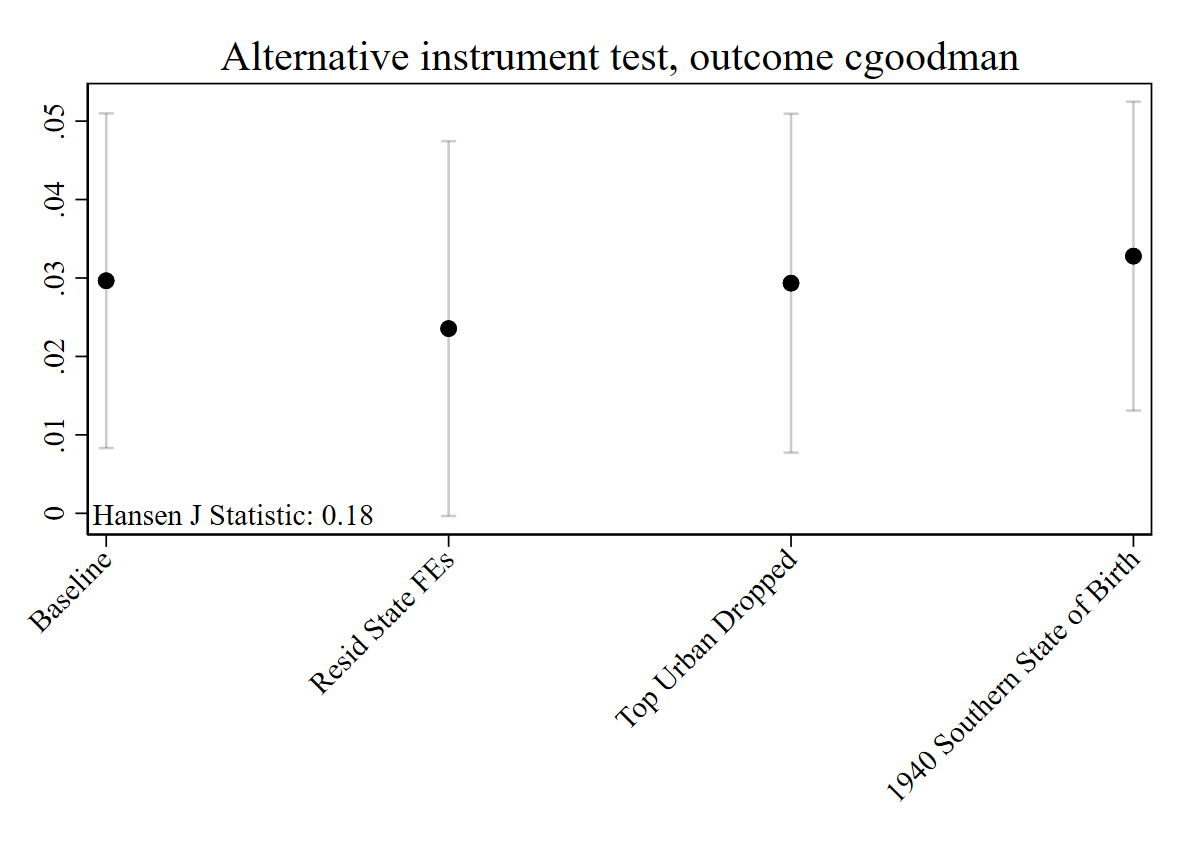
\includegraphics[width=.8\textwidth]{figures/exogeneity_tests/D16_alt_inst_pooled_cgoodman_urban.png}
\end{figure}
\clearpage
\begin{figure}
	\centering
	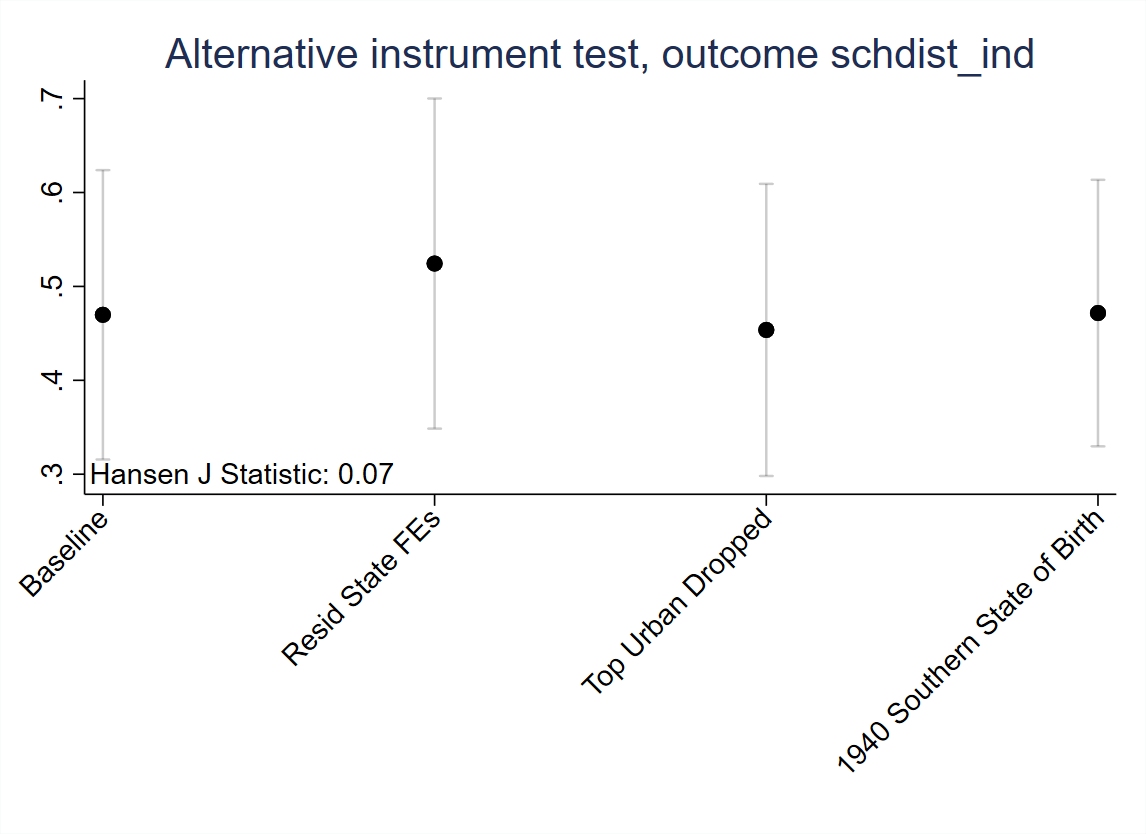
\includegraphics[width=.8\textwidth]{figures/exogeneity_tests/D16_alt_inst_pooled_schdist_ind_urban.png}
\end{figure}
\clearpage
\begin{figure}
	\centering
	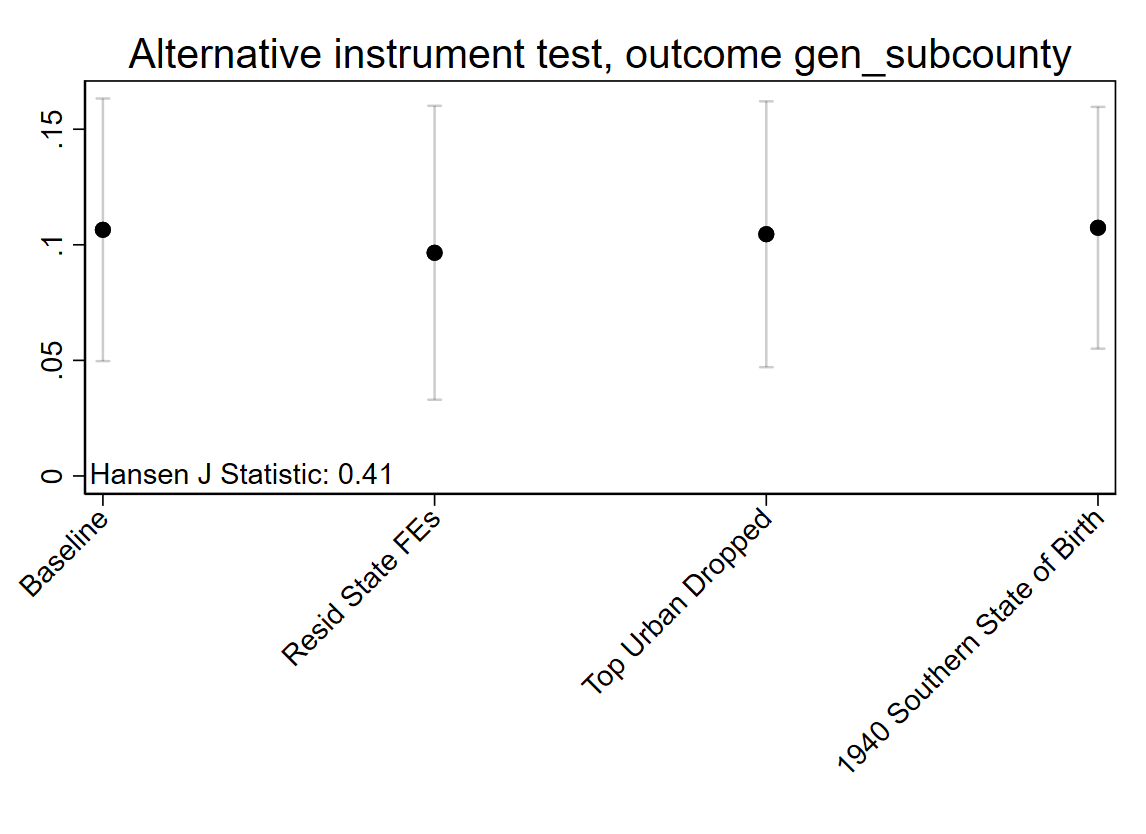
\includegraphics[width=.8\textwidth]{figures/exogeneity_tests/D16_alt_inst_pooled_gen_subcounty_urban.png}
\end{figure}
\clearpage
\begin{figure}
	\centering
	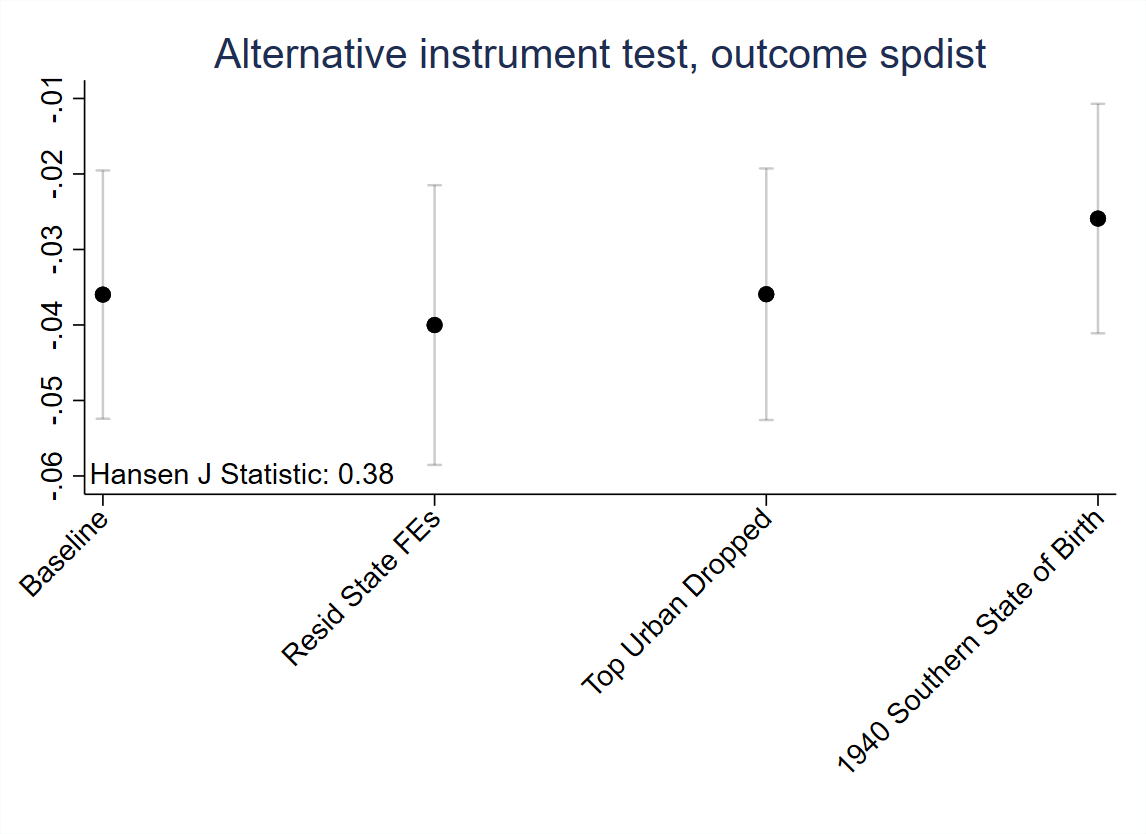
\includegraphics[width=.8\textwidth]{figures/exogeneity_tests/D16_alt_inst_pooled_spdist_urban.png}
\end{figure}
\clearpage

\clearpage
\begin{figure}
	\centering
	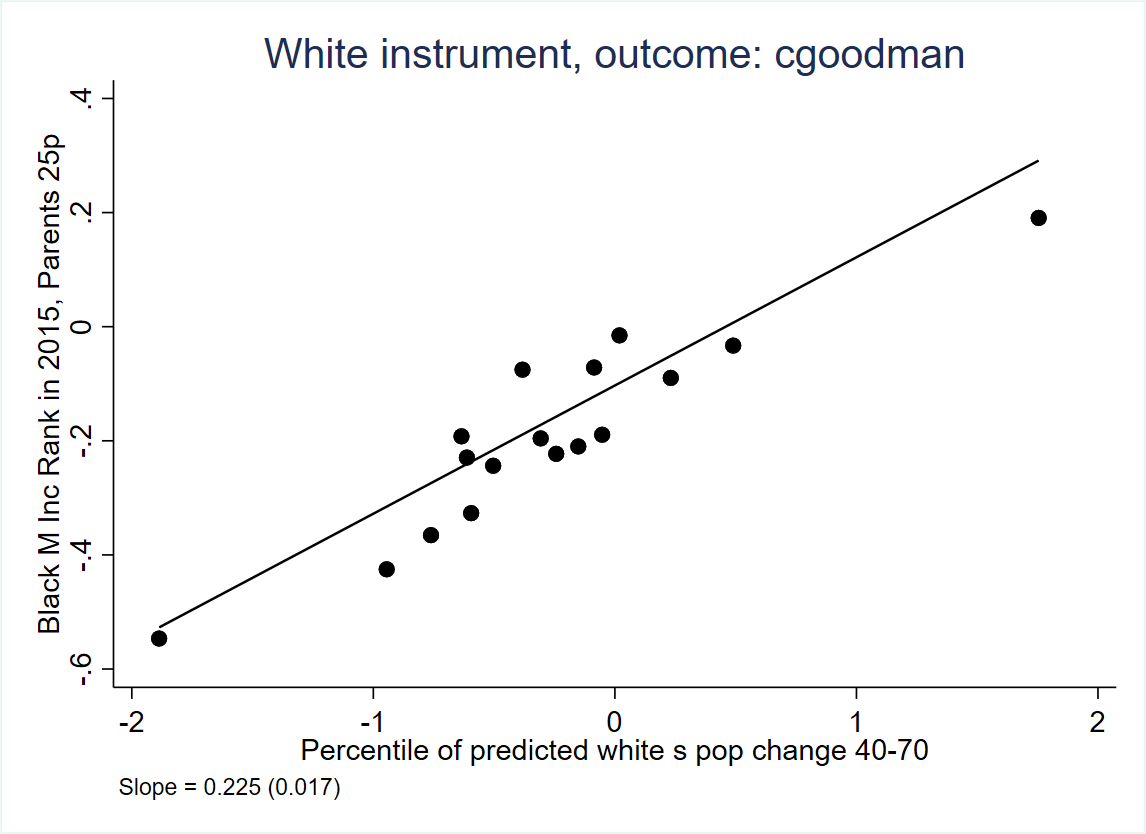
\includegraphics[width=.8\textwidth]{figures/exogeneity_tests/D14_cgoodman.png}
\end{figure}
\clearpage
\begin{figure}
	\centering
	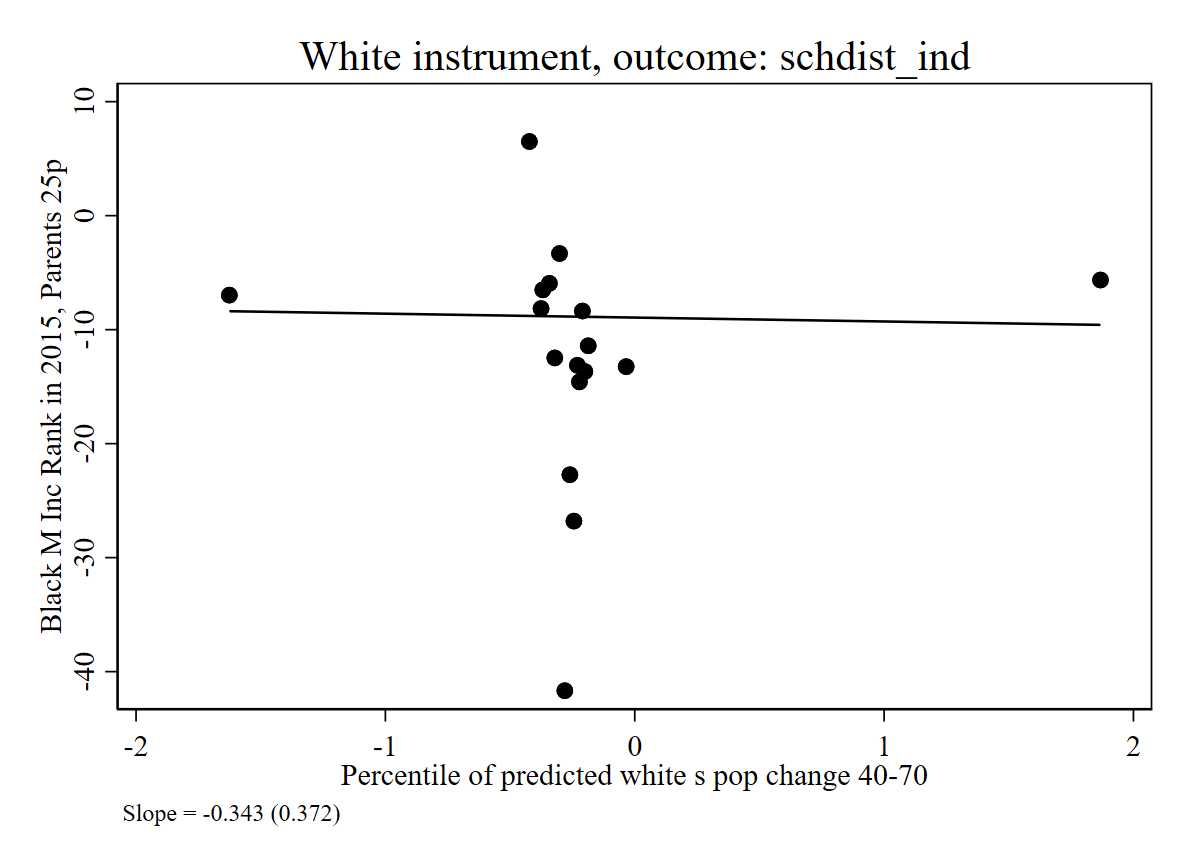
\includegraphics[width=.8\textwidth]{figures/exogeneity_tests/D14_schdist_ind.png}
\end{figure}
\clearpage
\begin{figure}
	\centering
	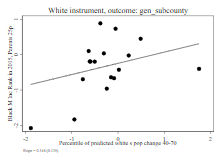
\includegraphics[width=.8\textwidth]{figures/exogeneity_tests/D14_gen_subcounty.png}
\end{figure}
\clearpage
\begin{figure}
	\centering
	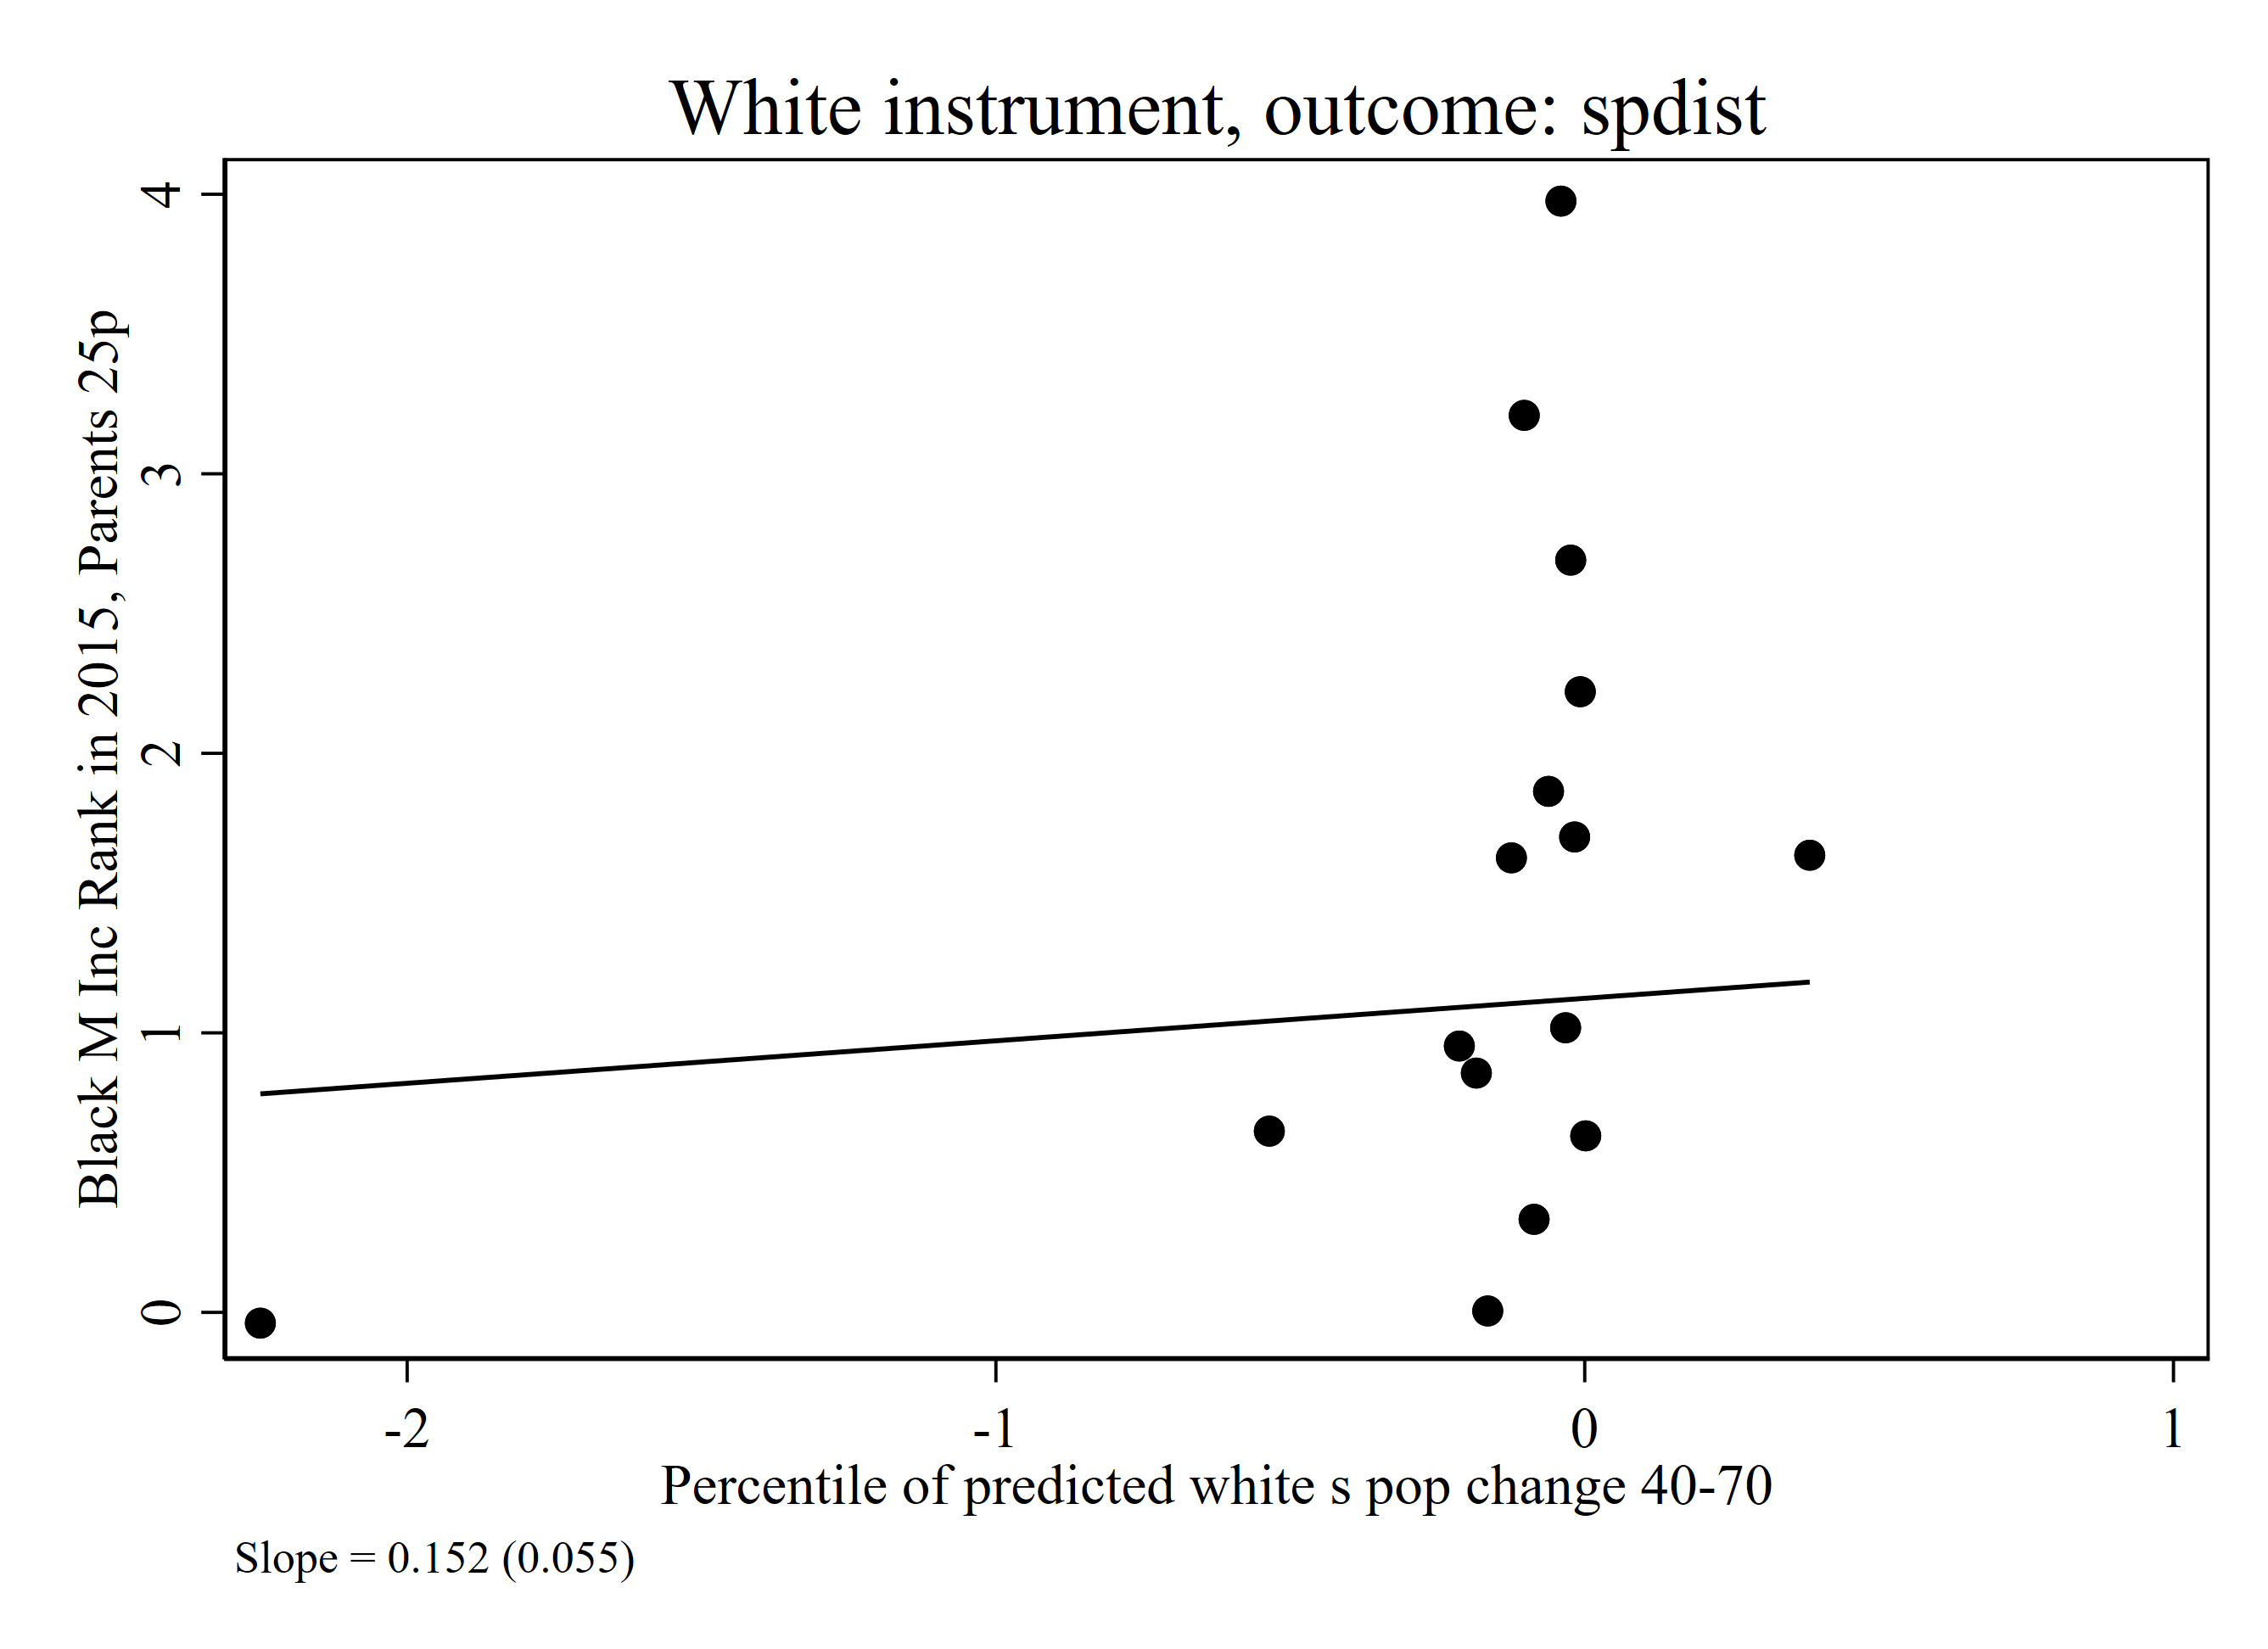
\includegraphics[width=.8\textwidth]{figures/exogeneity_tests/D14_spdist.png}
\end{figure}
\clearpage


\subsection{Baseline Instrument}
\begin{table}[htbp]\centering
\def\sym#1{\ifmmode^{#1}\else\(^{#1}\)\fi}
\caption{Outcome: cgoodman, Baseline Instrument}
\begin{tabular}{l*{4}{c}}
\toprule
                    & First Stage   &         OLS   &Reduced Form   &        2SLS   \\
                    &\multicolumn{1}{c}{(1)}   &\multicolumn{1}{c}{(2)}   &\multicolumn{1}{c}{(3)}   &\multicolumn{1}{c}{(4)}   \\
\midrule
Baseline Instrument &       3.044***&               &      0.0903** &               \\
                    &     (0.310)   &               &    (0.0402)   &               \\
\addlinespace
Percentage Point Change in Urban Black Population&               &      0.0235** &               &      0.0297** \\
                    &               &   (0.00904)   &               &    (0.0133)   \\
\midrule
F-Stat              &96.38800000000001   &               &               &               \\
Observations        &         130   &         130   &         130   &         130   \\
\bottomrule
\multicolumn{5}{l}{\footnotesize Standard errors in parentheses}\\
\multicolumn{5}{l}{\footnotesize * p<0.10, ** p<0.05, *** p<0.01}\\
\end{tabular}
\end{table}


\begin{table}[htbp]\centering
\def\sym#1{\ifmmode^{#1}\else\(^{#1}\)\fi}
\caption{Outcome: schdist\_ind, Baseline Instrument}
\begin{tabular}{l*{4}{c}}
\toprule
                    & First Stage   &         OLS   &Reduced Form   &        2SLS   \\
                    &\multicolumn{1}{c}{(1)}   &\multicolumn{1}{c}{(2)}   &\multicolumn{1}{c}{(3)}   &\multicolumn{1}{c}{(4)}   \\
\midrule
Baseline Instrument &       3.464***&               &       4.489***&               \\
                    &     (0.418)   &               &     (1.201)   &               \\
\addlinespace
Percentage Point Change in Urban Black Population&               &       1.047***&               &       1.296***\\
                    &               &     (0.255)   &               &     (0.326)   \\
\midrule
F-Stat              &      68.633   &               &               &               \\
Observations        &         130   &         130   &         130   &         130   \\
\bottomrule
\multicolumn{5}{l}{\footnotesize Standard errors in parentheses}\\
\multicolumn{5}{l}{\footnotesize * p<0.10, ** p<0.05, *** p<0.01}\\
\end{tabular}
\end{table}

\clearpage
\begin{table}[htbp]\centering
\def\sym#1{\ifmmode^{#1}\else\(^{#1}\)\fi}
\caption{Outcome: gen\_subcounty, Baseline Instrument}
\begin{tabular}{l*{4}{c}}
\toprule
                    & First Stage   &         OLS   &Reduced Form   &        2SLS   \\
                    &\multicolumn{1}{c}{(1)}   &\multicolumn{1}{c}{(2)}   &\multicolumn{1}{c}{(3)}   &\multicolumn{1}{c}{(4)}   \\
\midrule
Baseline Instrument &       3.464***&               &       0.473***&               \\
                    &     (0.418)   &               &     (0.113)   &               \\
\addlinespace
Percentage Point Change in Urban Black Population&               &      0.0877***&               &       0.136***\\
                    &               &    (0.0224)   &               &    (0.0319)   \\
\midrule
F-Stat              &      68.633   &               &               &               \\
Observations        &         130   &         130   &         130   &         130   \\
\bottomrule
\multicolumn{5}{l}{\footnotesize Standard errors in parentheses}\\
\multicolumn{5}{l}{\footnotesize * p<0.10, ** p<0.05, *** p<0.01}\\
\end{tabular}
\end{table}


\begin{table}[htbp]\centering
\def\sym#1{\ifmmode^{#1}\else\(^{#1}\)\fi}
\caption{Outcome: spdist, Baseline Instrument}
\begin{tabular}{l*{4}{c}}
\toprule
                    & First Stage   &         OLS   &Reduced Form   &        2SLS   \\
                    &\multicolumn{1}{c}{(1)}   &\multicolumn{1}{c}{(2)}   &\multicolumn{1}{c}{(3)}   &\multicolumn{1}{c}{(4)}   \\
\midrule
Baseline Instrument &       3.464***&               &     -0.0966   &               \\
                    &     (0.418)   &               &    (0.0989)   &               \\
\addlinespace
Percentage Point Change in Urban Black Population&               &     -0.0651***&               &     -0.0279   \\
                    &               &    (0.0231)   &               &    (0.0268)   \\
\midrule
F-Stat              &      68.633   &               &               &               \\
Observations        &         130   &         130   &         130   &         130   \\
\bottomrule
\multicolumn{5}{l}{\footnotesize Standard errors in parentheses}\\
\multicolumn{5}{l}{\footnotesize * p<0.10, ** p<0.05, *** p<0.01}\\
\end{tabular}
\end{table}

\clearpage

\subsection{Resid State FEs Instrument}
\begin{table}[htbp]\centering
\def\sym#1{\ifmmode^{#1}\else\(^{#1}\)\fi}
\caption{Outcome: cgoodman, Resid State FE Instrument}
\begin{tabular}{l*{4}{c}}
\toprule
                    & First Stage   &         OLS   &Reduced Form   &        2SLS   \\
                    &\multicolumn{1}{c}{(1)}   &\multicolumn{1}{c}{(2)}   &\multicolumn{1}{c}{(3)}   &\multicolumn{1}{c}{(4)}   \\
\midrule
Resid State FE Instrument&       3.264***&               &      0.0762   &               \\
                    &     (0.434)   &               &    (0.0493)   &               \\
\addlinespace
Percentage Point Change in Urban Black Population&               &      0.0235** &               &      0.0234   \\
                    &               &   (0.00904)   &               &    (0.0148)   \\
\midrule
F-Stat              &      56.532   &               &               &               \\
Observations        &         130   &         130   &         130   &         130   \\
\bottomrule
\multicolumn{5}{l}{\footnotesize Standard errors in parentheses}\\
\multicolumn{5}{l}{\footnotesize * p<0.10, ** p<0.05, *** p<0.01}\\
\end{tabular}
\end{table}


 \begin{tabular}{l*{4}{c}} \toprule
                    & First Stage   &         OLS   &Reduced Form   &        2SLS   \\
                    &\multicolumn{1}{c}{(1)}   &\multicolumn{1}{c}{(2)}   &\multicolumn{1}{c}{(3)}   &\multicolumn{1}{c}{(4)}   \\
\end{tabular}
Resid State FE Instrument&       5.180***&               &       2.762***&               \\
                    &     (0.910)   &               &     (0.785)   &               \\
\addlinespace
Percentage Point Change in Urban Black Population&               &       0.288***&               &       0.533***\\
                    &               &    (0.0840)   &               &     (0.140)   \\
\midrule
F-Stat              &       32.38   &               &               &               \\
Observations        &         130   &         130   &         130   &         130   \\
\bottomrule
\multicolumn{5}{l}{\footnotesize Standard errors in parentheses}\\
\multicolumn{5}{l}{\footnotesize * p<0.10, ** p<0.05, *** p<0.01}\\
\end{tabular}
\end{table}

\clearpage
 \begin{tabular}{l*{4}{c}} \toprule
                    & First Stage   &         OLS   &Reduced Form   &        2SLS   \\
                    &\multicolumn{1}{c}{(1)}   &\multicolumn{1}{c}{(2)}   &\multicolumn{1}{c}{(3)}   &\multicolumn{1}{c}{(4)}   \\
\end{tabular}
Resid State FE Instrument&       5.180***&               &       0.292***&               \\
                    &     (0.910)   &               &    (0.0866)   &               \\
\addlinespace
Percentage Point Change in Urban Black Population&               &      0.0257***&               &      0.0563***\\
                    &               &   (0.00827)   &               &    (0.0187)   \\
\midrule
F-Stat              &       32.38   &               &               &               \\
Observations        &         130   &         130   &         130   &         130   \\
\bottomrule
\multicolumn{5}{l}{\footnotesize Standard errors in parentheses}\\
\multicolumn{5}{l}{\footnotesize * p<0.10, ** p<0.05, *** p<0.01}\\
\end{tabular}
\end{table}


\begin{table}[htbp]\centering
\def\sym#1{\ifmmode^{#1}\else\(^{#1}\)\fi}
\caption{Outcome: spdist, Resid State FE Instrument}
\begin{tabular}{l*{4}{c}}
\toprule
                    & First Stage   &         OLS   &Reduced Form   &        2SLS   \\
                    &\multicolumn{1}{c}{(1)}   &\multicolumn{1}{c}{(2)}   &\multicolumn{1}{c}{(3)}   &\multicolumn{1}{c}{(4)}   \\
\midrule
Resid State FE Instrument&       3.264***&               &      -0.369***&               \\
                    &     (0.434)   &               &     (0.125)   &               \\
\addlinespace
Percentage Point Change in Urban Black Population&               &     -0.0861***&               &      -0.113***\\
                    &               &    (0.0236)   &               &    (0.0397)   \\
\midrule
F-Stat              &      56.532   &               &               &               \\
Observations        &         130   &         130   &         130   &         130   \\
\bottomrule
\multicolumn{5}{l}{\footnotesize Standard errors in parentheses}\\
\multicolumn{5}{l}{\footnotesize * p<0.10, ** p<0.05, *** p<0.01}\\
\end{tabular}
\end{table}

\clearpage


\subsection{Top Urban Dropped Instrument}
\begin{table}[htbp]\centering
\def\sym#1{\ifmmode^{#1}\else\(^{#1}\)\fi}
\caption{Outcome: cgoodman, Top Urban Dropped Instrument}
\begin{tabular}{l*{4}{c}}
\toprule
                    & First Stage   &         OLS   &Reduced Form   &        2SLS   \\
                    &\multicolumn{1}{c}{(1)}   &\multicolumn{1}{c}{(2)}   &\multicolumn{1}{c}{(3)}   &\multicolumn{1}{c}{(4)}   \\
\midrule
Top Urban Dropped Instrument&       3.459***&               &       0.150***&               \\
                    &     (0.488)   &               &    (0.0447)   &               \\
\addlinespace
Percentage Point Change in Urban Black Population&               &      0.0267***&               &      0.0433***\\
                    &               &   (0.00856)   &               &    (0.0140)   \\
\midrule
F-Stat              &      50.233   &               &               &               \\
Observations        &         130   &         130   &         130   &         130   \\
\bottomrule
\multicolumn{5}{l}{\footnotesize Standard errors in parentheses}\\
\multicolumn{5}{l}{\footnotesize * p<0.10, ** p<0.05, *** p<0.01}\\
\end{tabular}
\end{table}


 \begin{tabular}{l*{4}{c}} \toprule
                    & First Stage   &         OLS   &Reduced Form   &        2SLS   \\
                    &\multicolumn{1}{c}{(1)}   &\multicolumn{1}{c}{(2)}   &\multicolumn{1}{c}{(3)}   &\multicolumn{1}{c}{(4)}   \\
\end{tabular}
Top Urban Dropped Instrument&       3.459***&               &       1.345***&               \\
                    &     (0.488)   &               &     (0.417)   &               \\
\addlinespace
Percentage Point Change in Urban Black Population&               &       0.288***&               &       0.389***\\
                    &               &    (0.0840)   &               &     (0.112)   \\
\midrule
F-Stat              &      50.233   &               &               &               \\
Observations        &         130   &         130   &         130   &         130   \\
\bottomrule
\multicolumn{5}{l}{\footnotesize Standard errors in parentheses}\\
\multicolumn{5}{l}{\footnotesize * p<0.10, ** p<0.05, *** p<0.01}\\
\end{tabular}
\end{table}

\clearpage
\begin{table}[htbp]\centering
\def\sym#1{\ifmmode^{#1}\else\(^{#1}\)\fi}
\caption{Outcome: gen\_subcounty, Top Urban Dropped Instrument}
\begin{tabular}{l*{4}{c}}
\toprule
                    & First Stage   &         OLS   &Reduced Form   &        2SLS   \\
                    &\multicolumn{1}{c}{(1)}   &\multicolumn{1}{c}{(2)}   &\multicolumn{1}{c}{(3)}   &\multicolumn{1}{c}{(4)}   \\
\midrule
Top Urban Dropped Instrument&       3.459***&               &       0.453***&               \\
                    &     (0.488)   &               &     (0.117)   &               \\
\addlinespace
Percentage Point Change in Urban Black Population&               &      0.0877***&               &       0.131***\\
                    &               &    (0.0224)   &               &    (0.0318)   \\
\midrule
F-Stat              &      50.233   &               &               &               \\
Observations        &         130   &         130   &         130   &         130   \\
\bottomrule
\multicolumn{5}{l}{\footnotesize Standard errors in parentheses}\\
\multicolumn{5}{l}{\footnotesize * p<0.10, ** p<0.05, *** p<0.01}\\
\end{tabular}
\end{table}


 \begin{tabular}{l*{4}{c}} \toprule
                    & First Stage   &         OLS   &Reduced Form   &        2SLS   \\
                    &\multicolumn{1}{c}{(1)}   &\multicolumn{1}{c}{(2)}   &\multicolumn{1}{c}{(3)}   &\multicolumn{1}{c}{(4)}   \\
\end{tabular}
Top Urban Dropped Instrument&       3.459***&               &     -0.0780** &               \\
                    &     (0.488)   &               &    (0.0323)   &               \\
\addlinespace
Percentage Point Change in Urban Black Population&               &     -0.0268***&               &     -0.0226***\\
                    &               &   (0.00814)   &               &   (0.00844)   \\
\midrule
F-Stat              &      50.233   &               &               &               \\
Observations        &         130   &         130   &         130   &         130   \\
\bottomrule
\multicolumn{5}{l}{\footnotesize Standard errors in parentheses}\\
\multicolumn{5}{l}{\footnotesize * p<0.10, ** p<0.05, *** p<0.01}\\
\end{tabular}
\end{table}

\clearpage


\subsection{1940 Southern State of Birth Instrument}
 \begin{tabular}{l*{4}{c}} \toprule
                    & First Stage   &         OLS   &Reduced Form   &        2SLS   \\
                    &\multicolumn{1}{c}{(1)}   &\multicolumn{1}{c}{(2)}   &\multicolumn{1}{c}{(3)}   &\multicolumn{1}{c}{(4)}   \\
\end{tabular}
1940 Southern State of Birth Instrument&       10.05***&               &       0.145** &               \\
                    &     (1.202)   &               &    (0.0609)   &               \\
\addlinespace
Percentage Point Change in Urban Black Population&               &     0.00613*  &               &      0.0144** \\
                    &               &   (0.00349)   &               &   (0.00656)   \\
\midrule
F-Stat              &      69.879   &               &               &               \\
Observations        &         130   &         130   &         130   &         130   \\
\bottomrule
\multicolumn{5}{l}{\footnotesize Standard errors in parentheses}\\
\multicolumn{5}{l}{\footnotesize * p<0.10, ** p<0.05, *** p<0.01}\\
\end{tabular}
\end{table}


 \begin{tabular}{l*{4}{c}} \toprule
                    & First Stage   &         OLS   &Reduced Form   &        2SLS   \\
                    &\multicolumn{1}{c}{(1)}   &\multicolumn{1}{c}{(2)}   &\multicolumn{1}{c}{(3)}   &\multicolumn{1}{c}{(4)}   \\
\end{tabular}
1940 Southern State of Birth Instrument&       10.05***&               &       4.410***&               \\
                    &     (1.202)   &               &     (1.344)   &               \\
\addlinespace
Percentage Point Change in Urban Black Population&               &       0.288***&               &       0.439***\\
                    &               &    (0.0840)   &               &     (0.114)   \\
\midrule
F-Stat              &      69.879   &               &               &               \\
Observations        &         130   &         130   &         130   &         130   \\
\bottomrule
\multicolumn{5}{l}{\footnotesize Standard errors in parentheses}\\
\multicolumn{5}{l}{\footnotesize * p<0.10, ** p<0.05, *** p<0.01}\\
\end{tabular}
\end{table}

\clearpage
 \begin{tabular}{l*{4}{c}} \toprule
                    & First Stage   &         OLS   &Reduced Form   &        2SLS   \\
                    &\multicolumn{1}{c}{(1)}   &\multicolumn{1}{c}{(2)}   &\multicolumn{1}{c}{(3)}   &\multicolumn{1}{c}{(4)}   \\
\end{tabular}
1940 Southern State of Birth Instrument&       10.05***&               &       0.436***&               \\
                    &     (1.202)   &               &     (0.126)   &               \\
\addlinespace
Percentage Point Change in Urban Black Population&               &      0.0257***&               &      0.0433***\\
                    &               &   (0.00827)   &               &    (0.0131)   \\
\midrule
F-Stat              &      69.879   &               &               &               \\
Observations        &         130   &         130   &         130   &         130   \\
\bottomrule
\multicolumn{5}{l}{\footnotesize Standard errors in parentheses}\\
\multicolumn{5}{l}{\footnotesize * p<0.10, ** p<0.05, *** p<0.01}\\
\end{tabular}
\end{table}


\begin{table}[htbp]\centering
\def\sym#1{\ifmmode^{#1}\else\(^{#1}\)\fi}
\caption{Outcome: spdist, 1940 Southern State of Birth Instrument}
\begin{tabular}{l*{4}{c}}
\toprule
                    & First Stage   &         OLS   &Reduced Form   &        2SLS   \\
                    &\multicolumn{1}{c}{(1)}   &\multicolumn{1}{c}{(2)}   &\multicolumn{1}{c}{(3)}   &\multicolumn{1}{c}{(4)}   \\
\midrule
1940 Southern State of Birth Instrument&       10.05***&               &      -0.113   &               \\
                    &     (1.202)   &               &     (0.283)   &               \\
\addlinespace
Percentage Point Change in Urban Black Population&               &     -0.0651***&               &     -0.0113   \\
                    &               &    (0.0231)   &               &    (0.0270)   \\
\midrule
F-Stat              &      69.879   &               &               &               \\
Observations        &         130   &         130   &         130   &         130   \\
\bottomrule
\multicolumn{5}{l}{\footnotesize Standard errors in parentheses}\\
\multicolumn{5}{l}{\footnotesize * p<0.10, ** p<0.05, *** p<0.01}\\
\end{tabular}
\end{table}


\clearpage


\subsection{European Migrant Instrument as Control}
 \begin{tabular}{l*{4}{c}} \toprule
                    & First Stage   &         OLS   &Reduced Form   &        2SLS   \\
                    &\multicolumn{1}{c}{(1)}   &\multicolumn{1}{c}{(2)}   &\multicolumn{1}{c}{(3)}   &\multicolumn{1}{c}{(4)}   \\
\end{tabular}
Predicted Percentage Point Change in Urban Black Population&       2.791***&               &     0.00542   &               \\
                    &     (0.525)   &               &    (0.0246)   &               \\
\addlinespace
Percentage Point Change in Urban Black Population&               &    -0.00401   &               &     0.00194   \\
                    &               &   (0.00482)   &               &   (0.00857)   \\
\midrule
F-Stat              &      28.304   &               &               &               \\
Observations        &         130   &         130   &         130   &         130   \\
\bottomrule
\multicolumn{5}{l}{\footnotesize Standard errors in parentheses}\\
\multicolumn{5}{l}{\footnotesize * p<0.10, ** p<0.05, *** p<0.01}\\
\end{tabular}
\end{table}


\begin{table}[htbp]\centering
\def\sym#1{\ifmmode^{#1}\else\(^{#1}\)\fi}
\caption{Outcome: schdist\_ind, Baseline Instrument with european migrant control}
\begin{tabular}{l*{4}{c}}
\toprule
                    & First Stage   &         OLS   &Reduced Form   &        2SLS   \\
                    &\multicolumn{1}{c}{(1)}   &\multicolumn{1}{c}{(2)}   &\multicolumn{1}{c}{(3)}   &\multicolumn{1}{c}{(4)}   \\
\midrule
Predicted Percentage Point Change in Urban Black Population&       2.280***&               &       2.848***&               \\
                    &     (0.442)   &               &     (1.064)   &               \\
\addlinespace
Percentage Point Change in Urban Black Population&               &       0.838***&               &       1.249***\\
                    &               &     (0.234)   &               &     (0.451)   \\
\midrule
F-Stat              &      26.582   &               &               &               \\
Observations        &         130   &         130   &         130   &         130   \\
\bottomrule
\multicolumn{5}{l}{\footnotesize Standard errors in parentheses}\\
\multicolumn{5}{l}{\footnotesize * p<0.10, ** p<0.05, *** p<0.01}\\
\end{tabular}
\end{table}

\clearpage
\begin{table}[htbp]\centering
\def\sym#1{\ifmmode^{#1}\else\(^{#1}\)\fi}
\caption{Outcome: gen\_subcounty, Baseline Instrument with european migrant control}
\begin{tabular}{l*{4}{c}}
\toprule
                    & First Stage   &         OLS   &Reduced Form   &        2SLS   \\
                    &\multicolumn{1}{c}{(1)}   &\multicolumn{1}{c}{(2)}   &\multicolumn{1}{c}{(3)}   &\multicolumn{1}{c}{(4)}   \\
\midrule
Predicted Percentage Point Change in Urban Black Population&       2.791***&               &       0.423***&               \\
                    &     (0.525)   &               &     (0.120)   &               \\
\addlinespace
Percentage Point Change in Urban Black Population&               &      0.0794***&               &       0.151***\\
                    &               &    (0.0218)   &               &    (0.0449)   \\
\midrule
F-Stat              &      28.304   &               &               &               \\
Observations        &         130   &         130   &         130   &         130   \\
\bottomrule
\multicolumn{5}{l}{\footnotesize Standard errors in parentheses}\\
\multicolumn{5}{l}{\footnotesize * p<0.10, ** p<0.05, *** p<0.01}\\
\end{tabular}
\end{table}


\begin{table}[htbp]\centering
\def\sym#1{\ifmmode^{#1}\else\(^{#1}\)\fi}
\caption{Outcome: spdist, Baseline Instrument with european migrant control}
\begin{tabular}{l*{4}{c}}
\toprule
                    & First Stage   &         OLS   &Reduced Form   &        2SLS   \\
                    &\multicolumn{1}{c}{(1)}   &\multicolumn{1}{c}{(2)}   &\multicolumn{1}{c}{(3)}   &\multicolumn{1}{c}{(4)}   \\
\midrule
Predicted Percentage Point Change in Urban Black Population&       2.280***&               &     -0.0730   &               \\
                    &     (0.442)   &               &     (0.102)   &               \\
\addlinespace
Percentage Point Change in Urban Black Population&               &     -0.0525*  &               &     -0.0320   \\
                    &               &    (0.0268)   &               &    (0.0429)   \\
\midrule
F-Stat              &      26.582   &               &               &               \\
Observations        &         130   &         130   &         130   &         130   \\
\bottomrule
\multicolumn{5}{l}{\footnotesize Standard errors in parentheses}\\
\multicolumn{5}{l}{\footnotesize * p<0.10, ** p<0.05, *** p<0.01}\\
\end{tabular}
\end{table}


\clearpage


\subsection{Southern White Migration Instrument as Control}
 \begin{tabular}{l*{4}{c}} \toprule
                    & First Stage   &         OLS   &Reduced Form   &        2SLS   \\
                    &\multicolumn{1}{c}{(1)}   &\multicolumn{1}{c}{(2)}   &\multicolumn{1}{c}{(3)}   &\multicolumn{1}{c}{(4)}   \\
\end{tabular}
Predicted Percentage Point Change in Urban Black Population&       3.461***&               &      0.0281*  &               \\
                    &     (0.419)   &               &    (0.0147)   &               \\
\addlinespace
Percentage Point Change in Urban Black Population&               &     0.00432   &               &     0.00811** \\
                    &               &   (0.00317)   &               &   (0.00400)   \\
\midrule
F-Stat              &68.28700000000001   &               &               &               \\
Observations        &         130   &         130   &         130   &         130   \\
\bottomrule
\multicolumn{5}{l}{\footnotesize Standard errors in parentheses}\\
\multicolumn{5}{l}{\footnotesize * p<0.10, ** p<0.05, *** p<0.01}\\
\end{tabular}
\end{table}


\begin{table}[htbp]\centering
\def\sym#1{\ifmmode^{#1}\else\(^{#1}\)\fi}
\caption{Outcome: schdist\_ind, Baseline Instrument with european migrant control}
\begin{tabular}{l*{4}{c}}
\toprule
                    & First Stage   &         OLS   &Reduced Form   &        2SLS   \\
                    &\multicolumn{1}{c}{(1)}   &\multicolumn{1}{c}{(2)}   &\multicolumn{1}{c}{(3)}   &\multicolumn{1}{c}{(4)}   \\
\midrule
Predicted Percentage Point Change in Urban Black Population&       3.461***&               &       4.197***&               \\
                    &     (0.419)   &               &     (1.254)   &               \\
\addlinespace
Percentage Point Change in Urban Black Population&               &       1.005***&               &       1.213***\\
                    &               &     (0.258)   &               &     (0.338)   \\
\midrule
F-Stat              &68.28700000000001   &               &               &               \\
Observations        &         130   &         130   &         130   &         130   \\
\bottomrule
\multicolumn{5}{l}{\footnotesize Standard errors in parentheses}\\
\multicolumn{5}{l}{\footnotesize * p<0.10, ** p<0.05, *** p<0.01}\\
\end{tabular}
\end{table}

\clearpage
\begin{table}[htbp]\centering
\def\sym#1{\ifmmode^{#1}\else\(^{#1}\)\fi}
\caption{Outcome: gen\_subcounty, Baseline Instrument with european migrant control}
\begin{tabular}{l*{4}{c}}
\toprule
                    & First Stage   &         OLS   &Reduced Form   &        2SLS   \\
                    &\multicolumn{1}{c}{(1)}   &\multicolumn{1}{c}{(2)}   &\multicolumn{1}{c}{(3)}   &\multicolumn{1}{c}{(4)}   \\
\midrule
Predicted Percentage Point Change in Urban Black Population&       3.461***&               &       0.459***&               \\
                    &     (0.419)   &               &     (0.111)   &               \\
\addlinespace
Percentage Point Change in Urban Black Population&               &      0.0855***&               &       0.133***\\
                    &               &    (0.0226)   &               &    (0.0305)   \\
\midrule
F-Stat              &68.28700000000001   &               &               &               \\
Observations        &         130   &         130   &         130   &         130   \\
\bottomrule
\multicolumn{5}{l}{\footnotesize Standard errors in parentheses}\\
\multicolumn{5}{l}{\footnotesize * p<0.10, ** p<0.05, *** p<0.01}\\
\end{tabular}
\end{table}


\begin{table}[htbp]\centering
\def\sym#1{\ifmmode^{#1}\else\(^{#1}\)\fi}
\caption{Outcome: spdist, Baseline Instrument with european migrant control}
\begin{tabular}{l*{4}{c}}
\toprule
                    & First Stage   &         OLS   &Reduced Form   &        2SLS   \\
                    &\multicolumn{1}{c}{(1)}   &\multicolumn{1}{c}{(2)}   &\multicolumn{1}{c}{(3)}   &\multicolumn{1}{c}{(4)}   \\
\midrule
Predicted Percentage Point Change in Urban Black Population&       3.461***&               &     -0.0830   &               \\
                    &     (0.419)   &               &    (0.0964)   &               \\
\addlinespace
Percentage Point Change in Urban Black Population&               &     -0.0633***&               &     -0.0240   \\
                    &               &    (0.0232)   &               &    (0.0260)   \\
\midrule
F-Stat              &68.28700000000001   &               &               &               \\
Observations        &         130   &         130   &         130   &         130   \\
\bottomrule
\multicolumn{5}{l}{\footnotesize Standard errors in parentheses}\\
\multicolumn{5}{l}{\footnotesize * p<0.10, ** p<0.05, *** p<0.01}\\
\end{tabular}
\end{table}


\clearpage

\section{Total Populations}
\subsection{GM\_hat on all covariates}
{
\def\sym#1{\ifmmode^{#1}\else\(^{#1}\)\fi}
\begin{tabular}{l*{5}{c}}
\toprule
          &\multicolumn{1}{c}{1940-1970 Pooled}&\multicolumn{1}{c}{1940-1950}&\multicolumn{1}{c}{1950-1960}&\multicolumn{1}{c}{1960-1970}&\multicolumn{1}{c}{Stacked}\\
\midrule
mfg\_lfshare&    -0.00         &     0.03\sym{***}&     0.01\sym{***}&    -0.00         &     0.01\sym{***}\\
          &   (0.00)         &   (0.01)         &   (0.00)         &   (0.00)         &   (0.00)         \\
\addlinespace
blackmig3539&     4.64\sym{***}&     1.31         &     4.42\sym{***}&     5.37\sym{***}&     3.40\sym{***}\\
          &   (0.86)         &   (1.99)         &   (0.34)         &   (0.68)         &   (0.94)         \\
\addlinespace
frac\_land &     0.49         &     0.73         &     0.16         &     0.15         &     0.35         \\
          &   (0.28)         &   (0.50)         &   (0.14)         &   (0.23)         &   (0.26)         \\
\addlinespace
transpo\_cost\_1920&    -0.00         &     0.00         &    -0.00         &     0.01         &     0.00         \\
          &   (0.01)         &   (0.04)         &   (0.01)         &   (0.01)         &   (0.02)         \\
\addlinespace
coastal   &    -0.12         &    -0.35\sym{*}  &    -0.06         &    -0.09         &    -0.17         \\
          &   (0.10)         &   (0.17)         &   (0.05)         &   (0.07)         &   (0.10)         \\
\addlinespace
avg\_precip&    -0.01\sym{*}  &     0.00         &     0.00         &    -0.00         &     0.00         \\
          &   (0.00)         &   (0.00)         &   (0.00)         &   (0.00)         &   (0.00)         \\
\addlinespace
avg\_temp  &    -0.00         &    -0.00         &    -0.00         &    -0.00         &    -0.00         \\
          &   (0.00)         &   (0.00)         &   (0.00)         &   (0.00)         &   (0.00)         \\
\addlinespace
n\_wells   &    -0.00         &    -0.00         &    -0.00         &    -0.00\sym{*}  &    -0.00\sym{*}  \\
          &   (0.00)         &   (0.00)         &   (0.00)         &   (0.00)         &   (0.00)         \\
\addlinespace
totfrac\_in\_main\_city&    -0.25         &     0.24         &     0.16         &    -0.20         &     0.07         \\
          &   (0.22)         &   (0.34)         &   (0.09)         &   (0.18)         &   (0.15)         \\
\addlinespace
urbfrac\_in\_main\_city&    -0.00\sym{***}&     0.00         &    -0.00         &    -0.00\sym{***}&    -0.00         \\
          &   (0.00)         &   (0.00)         &   (0.00)         &   (0.00)         &   (0.00)         \\
\addlinespace
m\_rr      &     0.00\sym{*}  &     0.00         &    -0.00         &     0.00         &     0.00         \\
          &   (0.00)         &   (0.00)         &   (0.00)         &   (0.00)         &   (0.00)         \\
\addlinespace
m\_rr\_sqm2 &   581.81         &  1992.38         &   882.01         &   508.58         &  1247.53         \\
          & (947.24)         &(1705.00)         & (504.70)         & (589.84)         &(1059.41)         \\
\addlinespace
reg2      &     0.10         &     0.51\sym{**} &     0.08         &     0.05         &     0.22\sym{**} \\
          &   (0.12)         &   (0.18)         &   (0.05)         &   (0.09)         &   (0.08)         \\
\addlinespace
reg3      &    -0.26         &     0.54         &     0.12         &    -0.35         &     0.14         \\
          &   (0.29)         &   (0.59)         &   (0.15)         &   (0.21)         &   (0.26)         \\
\addlinespace
reg4      &     0.29\sym{*}  &    -0.44         &    -0.12\sym{*}  &     0.14         &    -0.16         \\
          &   (0.13)         &   (0.24)         &   (0.06)         &   (0.09)         &   (0.11)         \\
\addlinespace
1940.decade&                  &                  &                  &                  &     0.00         \\
          &                  &                  &                  &                  &      (.)         \\
\addlinespace
1950.decade&                  &                  &                  &                  &     0.17\sym{*}  \\
          &                  &                  &                  &                  &   (0.08)         \\
\addlinespace
1960.decade&                  &                  &                  &                  &     0.02         \\
          &                  &                  &                  &                  &   (0.08)         \\
\bottomrule
\multicolumn{6}{l}{\footnotesize Standard errors in parentheses}\\
\multicolumn{6}{l}{\footnotesize \sym{*} \(p<0.05\), \sym{**} \(p<0.01\), \sym{***} \(p<0.001\)}\\
\end{tabular}
}

\clearpage
\subsection{Individual covariates on GM\_hat}
\begin{table}[htbp]\centering
\def\sym#1{\ifmmode^{#1}\else\(^{#1}\)\fi}
\caption{}
\begin{tabular}{l*{5}{c}}
\toprule
                &\multicolumn{1}{c}{1940-1970 Pooled}&\multicolumn{1}{c}{1940-1950}&\multicolumn{1}{c}{1950-1960}&\multicolumn{1}{c}{1960-1970}&\multicolumn{1}{c}{Stacked}\\
\midrule
mfg\_lfshare on GM\_hat&     1.47         &     2.88\sym{***}&    10.51\sym{***}&     3.22         &     2.75\sym{***}\\
                &   (1.76)         &   (0.86)         &   (2.93)         &   (2.21)         &   (0.80)         \\
\addlinespace
frac\_land on GM\_hat&    -0.00         &     0.04         &     0.23\sym{*}  &    -0.03         &     0.04\sym{*}  \\
                &   (0.05)         &   (0.02)         &   (0.10)         &   (0.09)         &   (0.02)         \\
\addlinespace
transpo\_cost\_1920 on GM\_hat&    -0.09         &    -0.06         &    -0.22         &    -0.08         &    -0.05         \\
                &   (0.15)         &   (0.12)         &   (0.38)         &   (0.20)         &   (0.10)         \\
\addlinespace
coastal on GM\_hat&    -0.02         &     0.01         &     0.16         &    -0.03         &     0.02         \\
                &   (0.07)         &   (0.04)         &   (0.12)         &   (0.10)         &   (0.04)         \\
\addlinespace
avg\_precip on GM\_hat&    -4.35\sym{**} &     0.38         &     4.09         &    -6.14\sym{**} &    -0.12         \\
                &   (1.57)         &   (0.64)         &   (3.05)         &   (2.26)         &   (0.75)         \\
\addlinespace
avg\_temp on GM\_hat&    -7.02         &    -1.05         &    -1.14         &    -9.28         &    -1.93         \\
                &   (3.62)         &   (2.08)         &   (7.95)         &   (4.79)         &   (2.23)         \\
\addlinespace
n\_wells on GM\_hat&   -65.59         &   -33.69         &  -108.98         &   -91.60         &   -37.15         \\
                &  (50.42)         &  (21.43)         &  (81.41)         &  (73.06)         &  (19.68)         \\
\addlinespace
totfrac\_in\_main\_city on GM\_hat&     0.02         &     0.07\sym{**} &     0.34\sym{***}&    -0.01         &     0.07\sym{**} \\
                &   (0.08)         &   (0.03)         &   (0.09)         &   (0.11)         &   (0.02)         \\
\addlinespace
urbfrac\_in\_main\_city on GM\_hat& -1359.17         &   253.30         &  -789.69         & -2022.67         &   -82.20         \\
                &(1426.77)         & (279.12)         &(1182.64)         &(2112.42)         & (312.79)         \\
\addlinespace
m\_rr on GM\_hat  &  5.1e+05\sym{*}  &  1.1e+05         &  3.3e+05         &  6.5e+05         &  1.7e+05         \\
                &(2.6e+05)         &(1.1e+05)         &(4.3e+05)         &(3.6e+05)         &(1.4e+05)         \\
\addlinespace
m\_rr\_sqm2 on GM\_hat&     0.00         &     0.00\sym{**} &     0.00\sym{**} &     0.00         &     0.00\sym{**} \\
                &   (0.00)         &   (0.00)         &   (0.00)         &   (0.00)         &   (0.00)         \\
\addlinespace
popc1940 on GM\_hat&  1.2e+06         &  6.7e+05\sym{*}  &  2.6e+06\sym{**} &  1.7e+06         &  8.1e+05\sym{**} \\
                &(7.2e+05)         &(2.9e+05)         &(9.5e+05)         &(1.2e+06)         &(2.5e+05)         \\
\addlinespace
pop1940 on GM\_hat&  4.4e+05         &  4.8e+05\sym{*}  &  2.6e+06\sym{**} &  1.7e+05         &  5.5e+05\sym{*}  \\
                &(6.8e+05)         &(2.4e+05)         &(9.2e+05)         &(1.0e+06)         &(2.3e+05)         \\
\bottomrule
\multicolumn{6}{l}{\footnotesize Standard errors in parentheses}\\
\multicolumn{6}{l}{\footnotesize \sym{*} \(p<0.05\), \sym{**} \(p<0.01\), \sym{***} \(p<0.001\)}\\
\end{tabular}
\end{table}

\clearpage
\subsection{Regressions}
\begin{landscape}
 \begin{table}[htbp]\centering \def\sym#1{\ifmmode^{#1}\else\(^{#1}\)\fi} \begin{threeparttable} \caption{Outcome variable cgoodman} \begin{tabular}{l*{11}{c}} \toprule
          &\multicolumn{5}{c}{Basic controls}                                   &\multicolumn{5}{c}{Robust controls}                                  \\\cmidrule(lr){2-6}\cmidrule(lr){7-11}
          &\multicolumn{1}{c}{(1)}&\multicolumn{1}{c}{(2)}&\multicolumn{1}{c}{(3)}&\multicolumn{1}{c}{(4)}&\multicolumn{1}{c}{(5)}&\multicolumn{1}{c}{(6)}&\multicolumn{1}{c}{(7)}&\multicolumn{1}{c}{(8)}&\multicolumn{1}{c}{(9)}&\multicolumn{1}{c}{(10)}\\
          &\multicolumn{1}{c}{1940-1970 Pooled}&\multicolumn{1}{c}{1940-1950}&\multicolumn{1}{c}{1950-1960}&\multicolumn{1}{c}{1960-1970}&\multicolumn{1}{c}{Stacked}&\multicolumn{1}{c}{1940-1970 Pooled}&\multicolumn{1}{c}{1940-1950}&\multicolumn{1}{c}{1950-1960}&\multicolumn{1}{c}{1960-1970}&\multicolumn{1}{c}{Stacked}\\
\cmidrule(lr){1-11}
\multicolumn{10}{l}{Panel A: First Stage}\\
\cmidrule(lr){1-11}
GM\_hat\_raw\_pp\_totpop&      2.87***&      0.71***&      1.45***&      0.77   &      0.77***&      1.20***&      0.25** &      1.23***&      0.68***&      0.11   \\
          &    (0.97)   &    (0.21)   &    (0.33)   &    (0.53)   &    (0.18)   &    (0.45)   &    (0.12)   &    (0.39)   &    (0.23)   &    (0.10)   \\
\midrule
F-Stat    &      8.81   &      11.8   &     19.59   &       2.1   &      17.4   &      7.22   &      4.33   &      9.77   &      9.09   &      1.43   \\
Observations&    449.00   &    449.00   &    449.00   &    449.00   &   1347.00   &    130.00   &    130.00   &    130.00   &    130.00   &    390.00   \\
\cmidrule[\heavyrulewidth](lr){1-11} \\ \cmidrule[\heavyrulewidth](lr){1-11}
\multicolumn{10}{l}{Panel B: OLS}\\
\cmidrule(lr){1-11}
GM\_raw\_pp\_totpop&     -0.01   &     -0.00   &     -0.01   &     -0.01   &     -0.01   &      0.01   &      0.03   &      0.01   &     -0.02** &      0.00   \\
          &    (0.01)   &    (0.01)   &    (0.01)   &    (0.01)   &    (0.01)   &    (0.02)   &    (0.02)   &    (0.02)   &    (0.01)   &    (0.01)   \\
\midrule
Observations&    449.00   &    449.00   &    449.00   &    449.00   &   1347.00   &    130.00   &    130.00   &    130.00   &    130.00   &    390.00   \\
\cmidrule[\heavyrulewidth](lr){1-11} \\ \cmidrule[\heavyrulewidth](lr){1-11}
\multicolumn{10}{l}{Panel C: Reduced Form}\\
\cmidrule(lr){1-11}
GM\_hat\_raw\_pp\_totpop&      0.07   &     -0.00   &      0.01   &      0.06   &      0.02   &      0.16***&      0.01   &     -0.01   &      0.00   &      0.01   \\
          &    (0.05)   &    (0.01)   &    (0.02)   &    (0.04)   &    (0.02)   &    (0.05)   &    (0.02)   &    (0.04)   &    (0.02)   &    (0.01)   \\
\midrule
Observations&    449.00   &    449.00   &    449.00   &    449.00   &   1347.00   &    130.00   &    130.00   &    130.00   &    130.00   &    390.00   \\
\cmidrule[\heavyrulewidth](lr){1-11} \\ \cmidrule[\heavyrulewidth](lr){1-11}
\multicolumn{10}{l}{Panel D: 2SLS}\\
\cmidrule(lr){1-11}
GM\_raw\_pp\_totpop&      0.02   &     -0.00   &      0.01   &      0.08   &      0.03   &      0.13** &      0.04   &     -0.01   &      0.00   &      0.07   \\
          &    (0.02)   &    (0.01)   &    (0.02)   &    (0.10)   &    (0.02)   &    (0.06)   &    (0.06)   &    (0.03)   &    (0.03)   &    (0.10)   \\
\midrule
Observations&    449.00   &    449.00   &    449.00   &    449.00   &   1347.00   &    130.00   &    130.00   &    130.00   &    130.00   &    390.00   \\
\hline\hline
\end{tabular}{\caption*{\begin{scriptsize}
Columns 1-4 include region fixed effects, column 5 includes region and decade fixed effects. Columns 6-7 include region fixed effects and all significant covariates from the corresponding balance table. Column 10 includes region and decade fixed effects and all significant covariates from the corresponding balance table. \(p<0.10\), ** \(p<0.05\), *** \(p<0.01\)
\end{scriptsize}}}
\end{threeparttable}
\end{table}

\clearpage
 \begin{table}[htbp]\centering \def\sym#1{\ifmmode^{#1}\else\(^{#1}\)\fi} \begin{threeparttable} \caption{Outcome variable schdist\_ind} \begin{tabular}{l*{11}{c}} \toprule
          &\multicolumn{5}{c}{Basic controls}                                   &\multicolumn{5}{c}{Robust controls}                                  \\\cmidrule(lr){2-6}\cmidrule(lr){7-11}
          &\multicolumn{1}{c}{(1)}&\multicolumn{1}{c}{(2)}&\multicolumn{1}{c}{(3)}&\multicolumn{1}{c}{(4)}&\multicolumn{1}{c}{(5)}&\multicolumn{1}{c}{(6)}&\multicolumn{1}{c}{(7)}&\multicolumn{1}{c}{(8)}&\multicolumn{1}{c}{(9)}&\multicolumn{1}{c}{(10)}\\
          &\multicolumn{1}{c}{1940-1970 Pooled}&\multicolumn{1}{c}{1940-1950}&\multicolumn{1}{c}{1950-1960}&\multicolumn{1}{c}{1960-1970}&\multicolumn{1}{c}{Stacked}&\multicolumn{1}{c}{1940-1970 Pooled}&\multicolumn{1}{c}{1940-1950}&\multicolumn{1}{c}{1950-1960}&\multicolumn{1}{c}{1960-1970}&\multicolumn{1}{c}{Stacked}\\
\cmidrule(lr){1-11}
\multicolumn{10}{l}{Panel A: First Stage}\\
\cmidrule(lr){1-11}
GM\_hat\_raw\_pp\_totpop&      2.87***&      0.71***&      1.45***&      0.77   &      0.77***&      0.83** &      0.20** &      0.98***&     -0.10   &      0.06   \\
          &    (0.97)   &    (0.21)   &    (0.33)   &    (0.53)   &    (0.18)   &    (0.38)   &    (0.09)   &    (0.25)   &    (0.67)   &    (0.08)   \\
\midrule
F-Stat    &      2.99   &      4.30   &      7.21   &      0.97   &      4.06   &     48.36   &     40.62   &     56.26   &      4.09   &     32.59   \\
Observations&    449.00   &    449.00   &    449.00   &    449.00   &   1347.00   &    449.00   &    449.00   &    449.00   &    449.00   &   1347.00   \\
\cmidrule[\heavyrulewidth](lr){1-11} \\ \cmidrule[\heavyrulewidth](lr){1-11}
\multicolumn{10}{l}{Panel B: OLS}\\
\cmidrule(lr){1-11}
GM\_raw\_pp\_totpop&      1.52***&      1.53***&      2.01***&      0.87***&      1.30***&     -0.91** &     -0.08   &     -0.29   &      0.66** &     -0.76***\\
          &    (0.29)   &    (0.22)   &    (0.30)   &    (0.29)   &    (0.27)   &    (0.37)   &    (0.34)   &    (0.42)   &    (0.27)   &    (0.16)   \\
\midrule
Observations&    449.00   &    449.00   &    449.00   &    449.00   &   1347.00   &    449.00   &    449.00   &    449.00   &    449.00   &   1347.00   \\
\cmidrule[\heavyrulewidth](lr){1-11} \\ \cmidrule[\heavyrulewidth](lr){1-11}
\multicolumn{10}{l}{Panel C: Reduced Form}\\
\cmidrule(lr){1-11}
GM\_hat\_raw\_pp\_totpop&      5.52***&      1.20***&      3.79***&      1.39** &      1.79***&     -4.00***&     -0.23   &      0.31   &     -0.50   &     -0.13   \\
          &    (1.82)   &    (0.43)   &    (1.02)   &    (0.71)   &    (0.37)   &    (1.46)   &    (0.25)   &    (0.80)   &    (0.86)   &    (0.16)   \\
\midrule
Observations&    449.00   &    449.00   &    449.00   &    449.00   &   1347.00   &    449.00   &    449.00   &    449.00   &    449.00   &   1347.00   \\
\cmidrule[\heavyrulewidth](lr){1-11} \\ \cmidrule[\heavyrulewidth](lr){1-11}
\multicolumn{10}{l}{Panel D: 2SLS}\\
\cmidrule(lr){1-11}
GM\_raw\_pp\_totpop&      1.92***&      1.68***&      2.60***&      1.81***&      2.32***&     -4.84*  &     -1.13   &      0.32   &      4.77   &     -2.40   \\
          &    (0.32)   &    (0.36)   &    (0.53)   &    (0.65)   &    (0.32)   &    (2.61)   &    (1.30)   &    (0.82)   &   (25.58)   &    (4.08)   \\
\midrule
Observations&    449.00   &    449.00   &    449.00   &    449.00   &   1347.00   &    449.00   &    449.00   &    449.00   &    449.00   &   1347.00   \\
\hline\hline
\end{tabular}{\caption*{\begin{scriptsize}
Columns 1-4 include region fixed effects, column 5 includes region and decade fixed effects. Columns 6-7 include region fixed effects and all significant covariates from the corresponding balance table. Column 10 includes region and decade fixed effects and all significant covariates from the corresponding balance table. \(p<0.10\), ** \(p<0.05\), *** \(p<0.01\)
\end{scriptsize}}}
\end{threeparttable}
\end{table}

\clearpage
 \begin{table}[htbp]\centering \def\sym#1{\ifmmode^{#1}\else\(^{#1}\)\fi} \begin{threeparttable} \caption{Outcome variable gen\_subcounty } \begin{tabular}{l*{11}{c}} \toprule
          &\multicolumn{5}{c}{Basic controls}                                   &\multicolumn{5}{c}{Robust controls}                                  \\\cmidrule(lr){2-6}\cmidrule(lr){7-11}
          &\multicolumn{1}{c}{(1)}&\multicolumn{1}{c}{(2)}&\multicolumn{1}{c}{(3)}&\multicolumn{1}{c}{(4)}&\multicolumn{1}{c}{(5)}&\multicolumn{1}{c}{(6)}&\multicolumn{1}{c}{(7)}&\multicolumn{1}{c}{(8)}&\multicolumn{1}{c}{(9)}&\multicolumn{1}{c}{(10)}\\
          &\multicolumn{1}{c}{1940-1970 Pooled}&\multicolumn{1}{c}{1940-1950}&\multicolumn{1}{c}{1950-1960}&\multicolumn{1}{c}{1960-1970}&\multicolumn{1}{c}{Stacked}&\multicolumn{1}{c}{1940-1970 Pooled}&\multicolumn{1}{c}{1940-1950}&\multicolumn{1}{c}{1950-1960}&\multicolumn{1}{c}{1960-1970}&\multicolumn{1}{c}{Stacked}\\
\cmidrule(lr){1-11}
\multicolumn{10}{l}{Panel A: First Stage}\\
\cmidrule(lr){1-11}
GM\_hat\_raw\_pp\_totpop&      1.53   &      0.50***&      2.20***&     -0.10   &      0.37***&      1.42   &      0.29***&      0.82** &      0.27   &      0.11   \\
          &    (1.25)   &    (0.14)   &    (0.49)   &    (0.67)   &    (0.14)   &    (1.03)   &    (0.09)   &    (0.33)   &    (0.58)   &    (0.10)   \\
\midrule
F-Stat    &       1.5   &     12.04   &     20.34   &       .02   &      6.71   &      1.89   &     10.65   &      6.08   &       .22   &      1.28   \\
Observations&    449.00   &    449.00   &    449.00   &    449.00   &   1347.00   &    449.00   &    130.00   &    130.00   &    449.00   &    390.00   \\
\cmidrule[\heavyrulewidth](lr){1-11} \\ \cmidrule[\heavyrulewidth](lr){1-11}
\multicolumn{10}{l}{Panel B: OLS}\\
\cmidrule(lr){1-11}
GM\_raw\_pp\_totpop&     -0.00   &      0.01   &     -0.03   &     -0.02   &     -0.01   &      0.01   &      0.03   &     -0.02   &     -0.02   &     -0.02   \\
          &    (0.02)   &    (0.02)   &    (0.03)   &    (0.01)   &    (0.01)   &    (0.02)   &    (0.03)   &    (0.03)   &    (0.02)   &    (0.02)   \\
\midrule
Observations&    449.00   &    449.00   &    449.00   &    449.00   &   1347.00   &    449.00   &    130.00   &    130.00   &    449.00   &    390.00   \\
\cmidrule[\heavyrulewidth](lr){1-11} \\ \cmidrule[\heavyrulewidth](lr){1-11}
\multicolumn{10}{l}{Panel C: Reduced Form}\\
\cmidrule(lr){1-11}
GM\_hat\_raw\_pp\_totpop&      0.29***&     -0.00   &      0.03   &      0.08   &      0.01   &      0.40***&      0.05   &      0.06   &      0.09   &      0.03   \\
          &    (0.09)   &    (0.02)   &    (0.08)   &    (0.07)   &    (0.01)   &    (0.11)   &    (0.03)   &    (0.11)   &    (0.07)   &    (0.02)   \\
\midrule
Observations&    449.00   &    449.00   &    449.00   &    449.00   &   1347.00   &    449.00   &    130.00   &    130.00   &    449.00   &    390.00   \\
\cmidrule[\heavyrulewidth](lr){1-11} \\ \cmidrule[\heavyrulewidth](lr){1-11}
\multicolumn{10}{l}{Panel D: 2SLS}\\
\cmidrule(lr){1-11}
GM\_raw\_pp\_totpop&      0.19   &     -0.00   &      0.01   &     -0.80   &      0.04   &      0.28   &      0.16   &      0.08   &      0.32   &      0.25   \\
          &    (0.17)   &    (0.04)   &    (0.04)   &    (5.44)   &    (0.04)   &    (0.21)   &    (0.13)   &    (0.14)   &    (0.78)   &    (0.29)   \\
\midrule
Observations&    449.00   &    449.00   &    449.00   &    449.00   &   1347.00   &    449.00   &    130.00   &    130.00   &    449.00   &    390.00   \\
\hline\hline
\end{tabular}{\caption*{\begin{scriptsize}
Columns 1-4 include region fixed effects, column 5 includes region and decade fixed effects. Columns 6-7 include region fixed effects and all significant covariates from the corresponding balance table. Column 10 includes region and decade fixed effects and all significant covariates from the corresponding balance table. \(p<0.10\), ** \(p<0.05\), *** \(p<0.01\)
\end{scriptsize}}}
\end{threeparttable}
\end{table}

\clearpage
 \begin{table}[htbp]\centering \def\sym#1{\ifmmode^{#1}\else\(^{#1}\)\fi} \begin{threeparttable} \caption{Outcome variable spdist} \begin{tabular}{l*{11}{c}} \toprule
          &\multicolumn{5}{c}{Basic controls}                                   &\multicolumn{5}{c}{Robust controls}                                  \\\cmidrule(lr){2-6}\cmidrule(lr){7-11}
          &\multicolumn{1}{c}{(1)}&\multicolumn{1}{c}{(2)}&\multicolumn{1}{c}{(3)}&\multicolumn{1}{c}{(4)}&\multicolumn{1}{c}{(5)}&\multicolumn{1}{c}{(6)}&\multicolumn{1}{c}{(7)}&\multicolumn{1}{c}{(8)}&\multicolumn{1}{c}{(9)}&\multicolumn{1}{c}{(10)}\\
          &\multicolumn{1}{c}{1940-1970 Pooled}&\multicolumn{1}{c}{1940-1950}&\multicolumn{1}{c}{1950-1960}&\multicolumn{1}{c}{1960-1970}&\multicolumn{1}{c}{Stacked}&\multicolumn{1}{c}{1940-1970 Pooled}&\multicolumn{1}{c}{1940-1950}&\multicolumn{1}{c}{1950-1960}&\multicolumn{1}{c}{1960-1970}&\multicolumn{1}{c}{Stacked}\\
\cmidrule(lr){1-11}
\multicolumn{10}{l}{Panel A: First Stage}\\
\cmidrule(lr){1-11}
GM\_hat\_raw\_pp\_totpop&      2.87***&      0.71***&      1.45***&      0.77   &      0.77***&      1.20***&      0.25** &      1.23***&      0.68***&      0.11   \\
          &    (0.97)   &    (0.21)   &    (0.33)   &    (0.53)   &    (0.18)   &    (0.45)   &    (0.12)   &    (0.39)   &    (0.23)   &    (0.10)   \\
\midrule
F-Stat    &      8.81   &      11.8   &     19.59   &       2.1   &      17.4   &      7.22   &      4.33   &      9.77   &      9.09   &      1.43   \\
Observations&    449.00   &    449.00   &    449.00   &    449.00   &   1347.00   &    130.00   &    130.00   &    130.00   &    130.00   &    390.00   \\
\cmidrule[\heavyrulewidth](lr){1-11} \\ \cmidrule[\heavyrulewidth](lr){1-11}
\multicolumn{10}{l}{Panel B: OLS}\\
\cmidrule(lr){1-11}
GM\_raw\_pp\_totpop&     -0.16***&     -0.15***&     -0.18***&     -0.14***&     -0.15***&     -0.09** &     -0.07*  &     -0.15*  &     -0.15***&     -0.05*  \\
          &    (0.02)   &    (0.03)   &    (0.04)   &    (0.04)   &    (0.02)   &    (0.04)   &    (0.04)   &    (0.07)   &    (0.03)   &    (0.03)   \\
\midrule
Observations&    449.00   &    449.00   &    449.00   &    449.00   &   1347.00   &    130.00   &    130.00   &    130.00   &    130.00   &    390.00   \\
\cmidrule[\heavyrulewidth](lr){1-11} \\ \cmidrule[\heavyrulewidth](lr){1-11}
\multicolumn{10}{l}{Panel C: Reduced Form}\\
\cmidrule(lr){1-11}
GM\_hat\_raw\_pp\_totpop&     -0.70***&     -0.13*  &     -0.30***&     -0.08   &     -0.14** &     -0.13   &      0.03   &     -0.15   &     -0.12** &      0.02   \\
          &    (0.14)   &    (0.07)   &    (0.07)   &    (0.14)   &    (0.06)   &    (0.16)   &    (0.06)   &    (0.16)   &    (0.06)   &    (0.03)   \\
\midrule
Observations&    449.00   &    449.00   &    449.00   &    449.00   &   1347.00   &    130.00   &    130.00   &    130.00   &    130.00   &    390.00   \\
\cmidrule[\heavyrulewidth](lr){1-11} \\ \cmidrule[\heavyrulewidth](lr){1-11}
\multicolumn{10}{l}{Panel D: 2SLS}\\
\cmidrule(lr){1-11}
GM\_raw\_pp\_totpop&     -0.24***&     -0.18** &     -0.21***&     -0.10   &     -0.18***&     -0.11   &      0.12   &     -0.12   &     -0.18*  &      0.14   \\
          &    (0.06)   &    (0.09)   &    (0.06)   &    (0.13)   &    (0.06)   &    (0.12)   &    (0.27)   &    (0.13)   &    (0.09)   &    (0.26)   \\
\midrule
Observations&    449.00   &    449.00   &    449.00   &    449.00   &   1347.00   &    130.00   &    130.00   &    130.00   &    130.00   &    390.00   \\
\hline\hline
\end{tabular}{\caption*{\begin{scriptsize}
Columns 1-4 include region fixed effects, column 5 includes region and decade fixed effects. Columns 6-7 include region fixed effects and all significant covariates from the corresponding balance table. Column 10 includes region and decade fixed effects and all significant covariates from the corresponding balance table. \(p<0.10\), ** \(p<0.05\), *** \(p<0.01\)
\end{scriptsize}}}
\end{threeparttable}
\end{table}

\clearpage
\end{landscape}

\section{Total Populations, Dcourt sample}
\subsection{GM\_hat on all covariates}
{
\def\sym#1{\ifmmode^{#1}\else\(^{#1}\)\fi}
\begin{tabular}{l*{5}{c}}
\toprule
          &\multicolumn{1}{c}{1940-1970 Pooled}&\multicolumn{1}{c}{1940-1950}&\multicolumn{1}{c}{1950-1960}&\multicolumn{1}{c}{1960-1970}&\multicolumn{1}{c}{Stacked}\\
\midrule
mfg\_lfshare&     0.00         &     0.04\sym{**} &     0.01\sym{*}  &     0.00         &     0.02\sym{***}\\
          &   (0.00)         &   (0.01)         &   (0.00)         &   (0.00)         &   (0.01)         \\
\addlinespace
blackmig3539&     2.98\sym{***}&    -0.91         &     4.29\sym{***}&     2.96\sym{*}  &     1.10         \\
          &   (0.83)         &   (2.57)         &   (0.80)         &   (1.14)         &   (1.70)         \\
\addlinespace
frac\_land &     0.50         &    -0.20         &    -0.09         &     0.29         &     0.05         \\
          &   (0.35)         &   (0.68)         &   (0.18)         &   (0.28)         &   (0.33)         \\
\addlinespace
transpo\_cost\_1920&     0.00         &    -0.02         &    -0.01         &     0.02         &    -0.00         \\
          &   (0.04)         &   (0.09)         &   (0.03)         &   (0.02)         &   (0.05)         \\
\addlinespace
coastal   &    -0.16         &    -0.16         &    -0.02         &    -0.14\sym{*}  &    -0.10         \\
          &   (0.08)         &   (0.26)         &   (0.07)         &   (0.05)         &   (0.13)         \\
\addlinespace
avg\_precip&    -0.01\sym{*}  &     0.00         &     0.00         &    -0.00         &     0.00         \\
          &   (0.00)         &   (0.01)         &   (0.00)         &   (0.00)         &   (0.00)         \\
\addlinespace
avg\_temp  &    -0.00         &    -0.00         &    -0.00         &     0.00         &    -0.00         \\
          &   (0.00)         &   (0.01)         &   (0.00)         &   (0.00)         &   (0.00)         \\
\addlinespace
n\_wells   &    -0.00\sym{**} &    -0.00         &    -0.00         &    -0.00\sym{***}&    -0.00         \\
          &   (0.00)         &   (0.00)         &   (0.00)         &   (0.00)         &   (0.00)         \\
\addlinespace
totfrac\_in\_main\_city&     0.55         &     2.09\sym{*}  &     0.50\sym{*}  &     0.36         &     1.15\sym{**} \\
          &   (0.37)         &   (0.88)         &   (0.25)         &   (0.23)         &   (0.43)         \\
\addlinespace
urbfrac\_in\_main\_city&    -0.43         &    -0.24         &    -0.05         &    -0.22         &    -0.15         \\
          &   (0.25)         &   (0.46)         &   (0.14)         &   (0.18)         &   (0.18)         \\
\addlinespace
m\_rr      &     0.00\sym{**} &     0.00         &    -0.00         &     0.00\sym{**} &     0.00         \\
          &   (0.00)         &   (0.00)         &   (0.00)         &   (0.00)         &   (0.00)         \\
\addlinespace
m\_rr\_sqm2 &  -137.29         &  1527.84         &  1004.55         &    61.66         &   753.76         \\
          &(1073.84)         &(2182.88)         & (647.90)         & (692.19)         &(1254.68)         \\
\addlinespace
reg2      &     0.18         &     0.42         &     0.03         &     0.15         &     0.24\sym{**} \\
          &   (0.12)         &   (0.22)         &   (0.07)         &   (0.08)         &   (0.09)         \\
\addlinespace
reg3      &     0.05         &     0.36         &     0.11         &     0.05         &     0.30         \\
          &   (0.39)         &   (0.70)         &   (0.17)         &   (0.30)         &   (0.33)         \\
\addlinespace
reg4      &     0.32         &    -0.60         &    -0.19         &     0.10         &    -0.21         \\
          &   (0.24)         &   (0.48)         &   (0.13)         &   (0.13)         &   (0.26)         \\
\addlinespace
1940.decade&                  &                  &                  &                  &     0.00         \\
          &                  &                  &                  &                  &      (.)         \\
\addlinespace
1950.decade&                  &                  &                  &                  &     0.08         \\
          &                  &                  &                  &                  &   (0.09)         \\
\addlinespace
1960.decade&                  &                  &                  &                  &    -0.14         \\
          &                  &                  &                  &                  &   (0.10)         \\
\bottomrule
\multicolumn{6}{l}{\footnotesize Standard errors in parentheses}\\
\multicolumn{6}{l}{\footnotesize \sym{*} \(p<0.05\), \sym{**} \(p<0.01\), \sym{***} \(p<0.001\)}\\
\end{tabular}
}

\clearpage
\subsection{Individual covariates on GM\_hat}
{
\def\sym#1{\ifmmode^{#1}\else\(^{#1}\)\fi}
\begin{tabular}{l*{5}{c}}
\toprule
                &\multicolumn{1}{c}{1940-1970 Pooled}&\multicolumn{1}{c}{1940-1950}&\multicolumn{1}{c}{1950-1960}&\multicolumn{1}{c}{1960-1970}&\multicolumn{1}{c}{Stacked}\\
\midrule
mfg\_lfshare on GM\_hat&     2.77         &     3.15\sym{*}  &     2.98         &     2.12         &     2.61\sym{**} \\
                &   (1.83)         &   (1.27)         &   (2.85)         &   (2.64)         &   (1.00)         \\
\addlinespace
blackmig3539 on GM\_hat&     0.14\sym{***}&     0.04         &     0.16\sym{***}&     0.14\sym{***}&     0.07\sym{*}  \\
                &   (0.02)         &   (0.03)         &   (0.01)         &   (0.02)         &   (0.03)         \\
\addlinespace
frac\_land on GM\_hat&     0.16         &     0.09         &     0.26\sym{*}  &     0.28         &     0.14\sym{**} \\
                &   (0.09)         &   (0.05)         &   (0.12)         &   (0.14)         &   (0.05)         \\
\addlinespace
transpo\_cost\_1920 on GM\_hat&    -0.21\sym{*}  &    -0.13         &    -0.36\sym{*}  &    -0.37\sym{*}  &    -0.19\sym{**} \\
                &   (0.11)         &   (0.09)         &   (0.15)         &   (0.15)         &   (0.06)         \\
\addlinespace
coastal on GM\_hat&     0.13         &     0.07         &     0.20\sym{*}  &     0.19         &     0.10\sym{**} \\
                &   (0.07)         &   (0.03)         &   (0.09)         &   (0.11)         &   (0.04)         \\
\addlinespace
avg\_precip on GM\_hat&     0.73         &     1.22         &     4.56         &     1.02         &     1.59         \\
                &   (1.97)         &   (1.26)         &   (2.70)         &   (2.96)         &   (1.12)         \\
\addlinespace
avg\_temp on GM\_hat&    -5.61         &    -2.63         &    -2.77         &    -7.76         &    -3.14         \\
                &   (4.66)         &   (2.85)         &   (4.67)         &   (7.19)         &   (2.42)         \\
\addlinespace
n\_wells on GM\_hat&   -56.10         &   -20.55         &   -25.35         &   -98.89         &   -30.00\sym{*}  \\
                &  (29.73)         &  (16.82)         &  (28.18)         &  (52.28)         &  (14.78)         \\
\addlinespace
totfrac\_in\_main\_city on GM\_hat&     0.22\sym{**} &     0.13\sym{**} &     0.32\sym{***}&     0.35\sym{**} &     0.18\sym{***}\\
                &   (0.07)         &   (0.05)         &   (0.08)         &   (0.11)         &   (0.04)         \\
\addlinespace
urbfrac\_in\_main\_city on GM\_hat&     0.04         &     0.02         &     0.10         &     0.08         &     0.04         \\
                &   (0.05)         &   (0.03)         &   (0.07)         &   (0.08)         &   (0.03)         \\
\addlinespace
m\_rr on GM\_hat  &  6.8e+05\sym{**} &  2.1e+05         &  5.1e+05         &  1.0e+06\sym{*}  &  3.6e+05\sym{*}  \\
                &(2.3e+05)         &(1.1e+05)         &(2.9e+05)         &(4.1e+05)         &(1.5e+05)         \\
\addlinespace
m\_rr\_sqm2 on GM\_hat&     0.00         &     0.00\sym{*}  &     0.00\sym{**} &     0.00         &     0.00\sym{**} \\
                &   (0.00)         &   (0.00)         &   (0.00)         &   (0.00)         &   (0.00)         \\
\addlinespace
popc1940 on GM\_hat&  2.1e+06\sym{**} &  1.0e+06\sym{*}  &  2.8e+06\sym{**} &  3.3e+06\sym{*}  &  1.6e+06\sym{***}\\
                &(7.9e+05)         &(4.8e+05)         &(1.0e+06)         &(1.3e+06)         &(4.6e+05)         \\
\addlinespace
pop1940 on GM\_hat&  2.4e+06\sym{**} &  1.2e+06\sym{*}  &  3.2e+06\sym{**} &  3.8e+06\sym{**} &  1.8e+06\sym{***}\\
                &(8.0e+05)         &(5.0e+05)         &(9.9e+05)         &(1.3e+06)         &(4.8e+05)         \\
\bottomrule
\multicolumn{6}{l}{\footnotesize Standard errors in parentheses}\\
\multicolumn{6}{l}{\footnotesize \sym{*} \(p<0.05\), \sym{**} \(p<0.01\), \sym{***} \(p<0.001\)}\\
\end{tabular}
}

\clearpage
\subsection{Regressions}
\begin{landscape}
 \begin{table}[htbp]\centering \def\sym#1{\ifmmode^{#1}\else\(^{#1}\)\fi} \begin{threeparttable} \caption{Outcome variable cgoodman} \begin{tabular}{l*{11}{c}} \toprule
          &\multicolumn{5}{c}{Basic controls}                                   &\multicolumn{5}{c}{Robust controls}                                  \\\cmidrule(lr){2-6}\cmidrule(lr){7-11}
          &\multicolumn{1}{c}{(1)}&\multicolumn{1}{c}{(2)}&\multicolumn{1}{c}{(3)}&\multicolumn{1}{c}{(4)}&\multicolumn{1}{c}{(5)}&\multicolumn{1}{c}{(6)}&\multicolumn{1}{c}{(7)}&\multicolumn{1}{c}{(8)}&\multicolumn{1}{c}{(9)}&\multicolumn{1}{c}{(10)}\\
          &\multicolumn{1}{c}{1940-1970 Pooled}&\multicolumn{1}{c}{1940-1950}&\multicolumn{1}{c}{1950-1960}&\multicolumn{1}{c}{1960-1970}&\multicolumn{1}{c}{Stacked}&\multicolumn{1}{c}{1940-1970 Pooled}&\multicolumn{1}{c}{1940-1950}&\multicolumn{1}{c}{1950-1960}&\multicolumn{1}{c}{1960-1970}&\multicolumn{1}{c}{Stacked}\\
\cmidrule(lr){1-11}
\multicolumn{10}{l}{Panel A: First Stage}\\
\cmidrule(lr){1-11}
GM\_hat\_raw\_pp\_totpop&      4.67***&      0.98***&      1.90***&      2.68***&      1.14***&      1.70***&      0.25** &      1.18***&      0.61** &      0.11   \\
          &    (1.07)   &    (0.28)   &    (0.32)   &    (0.79)   &    (0.26)   &    (0.65)   &    (0.12)   &    (0.38)   &    (0.26)   &    (0.10)   \\
\midrule
F-Stat    &     18.96   &      12.6   &      36.2   &     11.64   &     19.81   &      6.88   &      4.49   &      9.59   &      5.63   &      1.43   \\
Observations&    130.00   &    130.00   &    130.00   &    130.00   &    390.00   &    130.00   &    130.00   &    130.00   &    130.00   &    390.00   \\
\cmidrule[\heavyrulewidth](lr){1-11} \\ \cmidrule[\heavyrulewidth](lr){1-11}
\multicolumn{10}{l}{Panel B: OLS}\\
\cmidrule(lr){1-11}
GM\_raw\_pp\_totpop&      0.02***&      0.02** &      0.02** &      0.00   &      0.01** &      0.01   &      0.03   &      0.01   &     -0.02** &      0.00   \\
          &    (0.01)   &    (0.01)   &    (0.01)   &    (0.00)   &    (0.01)   &    (0.02)   &    (0.02)   &    (0.02)   &    (0.01)   &    (0.01)   \\
\midrule
Observations&    130.00   &    130.00   &    130.00   &    130.00   &    390.00   &    130.00   &    130.00   &    130.00   &    130.00   &    390.00   \\
\cmidrule[\heavyrulewidth](lr){1-11} \\ \cmidrule[\heavyrulewidth](lr){1-11}
\multicolumn{10}{l}{Panel C: Reduced Form}\\
\cmidrule(lr){1-11}
GM\_hat\_raw\_pp\_totpop&      0.13***&      0.02   &      0.04*  &      0.03   &      0.03***&      0.14***&      0.01   &     -0.02   &      0.00   &      0.01   \\
          &    (0.03)   &    (0.01)   &    (0.02)   &    (0.02)   &    (0.01)   &    (0.05)   &    (0.02)   &    (0.04)   &    (0.03)   &    (0.01)   \\
\midrule
Observations&    130.00   &    130.00   &    130.00   &    130.00   &    390.00   &    130.00   &    130.00   &    130.00   &    130.00   &    390.00   \\
\cmidrule[\heavyrulewidth](lr){1-11} \\ \cmidrule[\heavyrulewidth](lr){1-11}
\multicolumn{10}{l}{Panel D: 2SLS}\\
\cmidrule(lr){1-11}
GM\_raw\_pp\_totpop&      0.03***&      0.02*  &      0.02** &      0.01** &      0.02***&      0.08** &      0.04   &     -0.02   &      0.00   &      0.07   \\
          &    (0.01)   &    (0.01)   &    (0.01)   &    (0.01)   &    (0.01)   &    (0.04)   &    (0.06)   &    (0.03)   &    (0.04)   &    (0.10)   \\
\midrule
Observations&    130.00   &    130.00   &    130.00   &    130.00   &    390.00   &    130.00   &    130.00   &    130.00   &    130.00   &    390.00   \\
\hline\hline
\end{tabular}{\caption*{\begin{scriptsize}
Columns 1-4 include region fixed effects, column 5 includes region and decade fixed effects. Columns 6-7 include region fixed effects and all significant covariates from the corresponding balance table. Column 10 includes region and decade fixed effects and all significant covariates from the corresponding balance table. \(p<0.10\), ** \(p<0.05\), *** \(p<0.01\)
\end{scriptsize}}}
\end{threeparttable}
\end{table}

\clearpage
 \begin{table}[htbp]\centering \def\sym#1{\ifmmode^{#1}\else\(^{#1}\)\fi} \begin{threeparttable} \caption{Outcome variable schdist\_ind} \begin{tabular}{l*{11}{c}} \toprule
          &\multicolumn{5}{c}{Basic controls}                                   &\multicolumn{5}{c}{Robust controls}                                  \\\cmidrule(lr){2-6}\cmidrule(lr){7-11}
          &\multicolumn{1}{c}{(1)}&\multicolumn{1}{c}{(2)}&\multicolumn{1}{c}{(3)}&\multicolumn{1}{c}{(4)}&\multicolumn{1}{c}{(5)}&\multicolumn{1}{c}{(6)}&\multicolumn{1}{c}{(7)}&\multicolumn{1}{c}{(8)}&\multicolumn{1}{c}{(9)}&\multicolumn{1}{c}{(10)}\\
          &\multicolumn{1}{c}{1940-1970 Pooled}&\multicolumn{1}{c}{1940-1950}&\multicolumn{1}{c}{1950-1960}&\multicolumn{1}{c}{1960-1970}&\multicolumn{1}{c}{Stacked}&\multicolumn{1}{c}{1940-1970 Pooled}&\multicolumn{1}{c}{1940-1950}&\multicolumn{1}{c}{1950-1960}&\multicolumn{1}{c}{1960-1970}&\multicolumn{1}{c}{Stacked}\\
\cmidrule(lr){1-11}
\multicolumn{10}{l}{Panel A: First Stage}\\
\cmidrule(lr){1-11}
GM\_hat\_raw\_pp\_totpop&      4.67***&      0.98***&      1.90***&      2.68***&      1.14***&      1.70***&      0.25** &      1.18***&      0.61** &      0.11   \\
          &    (1.07)   &    (0.28)   &    (0.32)   &    (0.79)   &    (0.26)   &    (0.65)   &    (0.12)   &    (0.38)   &    (0.26)   &    (0.10)   \\
\midrule
F-Stat    &     18.96   &      12.6   &      36.2   &     11.64   &     19.81   &      6.88   &      4.49   &      9.59   &      5.63   &      1.43   \\
Observations&    130.00   &    130.00   &    130.00   &    130.00   &    390.00   &    130.00   &    130.00   &    130.00   &    130.00   &    390.00   \\
\cmidrule[\heavyrulewidth](lr){1-11} \\ \cmidrule[\heavyrulewidth](lr){1-11}
\multicolumn{10}{l}{Panel B: OLS}\\
\cmidrule(lr){1-11}
GM\_raw\_pp\_totpop&      0.90***&      1.07***&      1.17***&      0.41***&      0.74***&      0.10   &     -0.35   &      0.15   &      0.57***&     -0.42***\\
          &    (0.20)   &    (0.22)   &    (0.23)   &    (0.13)   &    (0.19)   &    (0.30)   &    (0.36)   &    (0.38)   &    (0.18)   &    (0.15)   \\
\midrule
Observations&    130.00   &    130.00   &    130.00   &    130.00   &    390.00   &    130.00   &    130.00   &    130.00   &    130.00   &    390.00   \\
\cmidrule[\heavyrulewidth](lr){1-11} \\ \cmidrule[\heavyrulewidth](lr){1-11}
\multicolumn{10}{l}{Panel C: Reduced Form}\\
\cmidrule(lr){1-11}
GM\_hat\_raw\_pp\_totpop&      5.12***&      1.43***&      3.41***&      1.60***&      1.66***&      0.27   &     -0.12   &      1.96** &      0.20   &      0.37*  \\
          &    (1.13)   &    (0.52)   &    (0.65)   &    (0.32)   &    (0.38)   &    (1.35)   &    (0.36)   &    (0.76)   &    (0.32)   &    (0.20)   \\
\midrule
Observations&    130.00   &    130.00   &    130.00   &    130.00   &    390.00   &    130.00   &    130.00   &    130.00   &    130.00   &    390.00   \\
\cmidrule[\heavyrulewidth](lr){1-11} \\ \cmidrule[\heavyrulewidth](lr){1-11}
\multicolumn{10}{l}{Panel D: 2SLS}\\
\cmidrule(lr){1-11}
GM\_raw\_pp\_totpop&      1.10***&      1.46***&      1.79***&      0.60***&      1.45***&      0.16   &     -0.48   &      1.66** &      0.32   &      3.27   \\
          &    (0.22)   &    (0.35)   &    (0.42)   &    (0.17)   &    (0.23)   &    (0.76)   &    (1.41)   &    (0.79)   &    (0.51)   &    (3.17)   \\
\midrule
Observations&    130.00   &    130.00   &    130.00   &    130.00   &    390.00   &    130.00   &    130.00   &    130.00   &    130.00   &    390.00   \\
\hline\hline
\end{tabular}{\caption*{\begin{scriptsize}
Columns 1-4 include region fixed effects, column 5 includes region and decade fixed effects. Columns 6-7 include region fixed effects and all significant covariates from the corresponding balance table. Column 10 includes region and decade fixed effects and all significant covariates from the corresponding balance table. \(p<0.10\), ** \(p<0.05\), *** \(p<0.01\)
\end{scriptsize}}}
\end{threeparttable}
\end{table}

\clearpage
 \begin{table}[htbp]\centering \def\sym#1{\ifmmode^{#1}\else\(^{#1}\)\fi} \begin{threeparttable} \caption{Outcome variable gen\_subcounty} \begin{tabular}{l*{11}{c}} \toprule
          &\multicolumn{5}{c}{Basic controls}                                   &\multicolumn{5}{c}{Robust controls}                                  \\\cmidrule(lr){2-6}\cmidrule(lr){7-11}
          &\multicolumn{1}{c}{(1)}&\multicolumn{1}{c}{(2)}&\multicolumn{1}{c}{(3)}&\multicolumn{1}{c}{(4)}&\multicolumn{1}{c}{(5)}&\multicolumn{1}{c}{(6)}&\multicolumn{1}{c}{(7)}&\multicolumn{1}{c}{(8)}&\multicolumn{1}{c}{(9)}&\multicolumn{1}{c}{(10)}\\
          &\multicolumn{1}{c}{1940-1970 Pooled}&\multicolumn{1}{c}{1940-1950}&\multicolumn{1}{c}{1950-1960}&\multicolumn{1}{c}{1960-1970}&\multicolumn{1}{c}{Stacked}&\multicolumn{1}{c}{1940-1970 Pooled}&\multicolumn{1}{c}{1940-1950}&\multicolumn{1}{c}{1950-1960}&\multicolumn{1}{c}{1960-1970}&\multicolumn{1}{c}{Stacked}\\
\cmidrule(lr){1-11}
\multicolumn{10}{l}{Panel A: First Stage}\\
\cmidrule(lr){1-11}
GM\_hat\_raw\_pp\_totpop&      4.67***&      0.98***&      1.90***&      2.68***&      1.14***&      1.70***&      0.25** &      1.18***&      0.61** &      0.11   \\
          &    (1.07)   &    (0.28)   &    (0.32)   &    (0.79)   &    (0.26)   &    (0.65)   &    (0.12)   &    (0.38)   &    (0.26)   &    (0.10)   \\
\midrule
F-Stat    &     18.96   &      12.6   &      36.2   &     11.64   &     19.81   &      6.88   &      4.49   &      9.59   &      5.63   &      1.43   \\
Observations&    130.00   &    130.00   &    130.00   &    130.00   &    390.00   &    130.00   &    130.00   &    130.00   &    130.00   &    390.00   \\
\cmidrule[\heavyrulewidth](lr){1-11} \\ \cmidrule[\heavyrulewidth](lr){1-11}
\multicolumn{10}{l}{Panel B: OLS}\\
\cmidrule(lr){1-11}
GM\_raw\_pp\_totpop&      0.07***&      0.07***&      0.07***&      0.03***&      0.05***&     -0.01   &      0.04   &     -0.02   &     -0.02   &     -0.02   \\
          &    (0.01)   &    (0.02)   &    (0.02)   &    (0.01)   &    (0.01)   &    (0.02)   &    (0.03)   &    (0.03)   &    (0.02)   &    (0.02)   \\
\midrule
Observations&    130.00   &    130.00   &    130.00   &    130.00   &    390.00   &    130.00   &    130.00   &    130.00   &    130.00   &    390.00   \\
\cmidrule[\heavyrulewidth](lr){1-11} \\ \cmidrule[\heavyrulewidth](lr){1-11}
\multicolumn{10}{l}{Panel C: Reduced Form}\\
\cmidrule(lr){1-11}
GM\_hat\_raw\_pp\_totpop&      0.48***&      0.09** &      0.19***&      0.18***&      0.11***&      0.37***&      0.04   &      0.05   &      0.10   &      0.03   \\
          &    (0.08)   &    (0.04)   &    (0.05)   &    (0.04)   &    (0.03)   &    (0.12)   &    (0.04)   &    (0.11)   &    (0.07)   &    (0.02)   \\
\midrule
Observations&    130.00   &    130.00   &    130.00   &    130.00   &    390.00   &    130.00   &    130.00   &    130.00   &    130.00   &    390.00   \\
\cmidrule[\heavyrulewidth](lr){1-11} \\ \cmidrule[\heavyrulewidth](lr){1-11}
\multicolumn{10}{l}{Panel D: 2SLS}\\
\cmidrule(lr){1-11}
GM\_raw\_pp\_totpop&      0.10***&      0.09***&      0.10***&      0.07***&      0.09***&      0.22*  &      0.16   &      0.04   &      0.16   &      0.23   \\
          &    (0.02)   &    (0.03)   &    (0.02)   &    (0.02)   &    (0.02)   &    (0.12)   &    (0.14)   &    (0.10)   &    (0.14)   &    (0.26)   \\
\midrule
Observations&    130.00   &    130.00   &    130.00   &    130.00   &    390.00   &    130.00   &    130.00   &    130.00   &    130.00   &    390.00   \\
\hline\hline
\end{tabular}{\caption*{\begin{scriptsize}
Columns 1-4 include region fixed effects, column 5 includes region and decade fixed effects. Columns 6-7 include region fixed effects and all significant covariates from the corresponding balance table. Column 10 includes region and decade fixed effects and all significant covariates from the corresponding balance table. \(p<0.10\), ** \(p<0.05\), *** \(p<0.01\)
\end{scriptsize}}}
\end{threeparttable}
\end{table}

\clearpage
 \begin{table}[htbp]\centering \def\sym#1{\ifmmode^{#1}\else\(^{#1}\)\fi} \begin{threeparttable} \caption{Outcome variable spdist} \begin{tabular}{l*{11}{c}} \toprule
          &\multicolumn{5}{c}{Basic controls}                                   &\multicolumn{5}{c}{Robust controls}                                  \\\cmidrule(lr){2-6}\cmidrule(lr){7-11}
          &\multicolumn{1}{c}{(1)}&\multicolumn{1}{c}{(2)}&\multicolumn{1}{c}{(3)}&\multicolumn{1}{c}{(4)}&\multicolumn{1}{c}{(5)}&\multicolumn{1}{c}{(6)}&\multicolumn{1}{c}{(7)}&\multicolumn{1}{c}{(8)}&\multicolumn{1}{c}{(9)}&\multicolumn{1}{c}{(10)}\\
          &\multicolumn{1}{c}{1940-1970 Pooled}&\multicolumn{1}{c}{1940-1950}&\multicolumn{1}{c}{1950-1960}&\multicolumn{1}{c}{1960-1970}&\multicolumn{1}{c}{Stacked}&\multicolumn{1}{c}{1940-1970 Pooled}&\multicolumn{1}{c}{1940-1950}&\multicolumn{1}{c}{1950-1960}&\multicolumn{1}{c}{1960-1970}&\multicolumn{1}{c}{Stacked}\\
\cmidrule(lr){1-11}
\multicolumn{10}{l}{Panel A: First Stage}\\
\cmidrule(lr){1-11}
GM\_hat\_raw\_pp\_totpop&      4.67***&      0.98***&      1.90***&      2.68***&      1.14***&      1.70***&      0.25** &      1.18***&      0.61** &      0.11   \\
          &    (1.07)   &    (0.28)   &    (0.32)   &    (0.79)   &    (0.26)   &    (0.65)   &    (0.12)   &    (0.38)   &    (0.26)   &    (0.10)   \\
\midrule
F-Stat    &     18.96   &      12.6   &      36.2   &     11.64   &     19.81   &      6.88   &      4.49   &      9.59   &      5.63   &      1.43   \\
Observations&    130.00   &    130.00   &    130.00   &    130.00   &    390.00   &    130.00   &    130.00   &    130.00   &    130.00   &    390.00   \\
\cmidrule[\heavyrulewidth](lr){1-11} \\ \cmidrule[\heavyrulewidth](lr){1-11}
\multicolumn{10}{l}{Panel B: OLS}\\
\cmidrule(lr){1-11}
GM\_raw\_pp\_totpop&     -0.08***&     -0.07***&     -0.12** &     -0.05***&     -0.07***&     -0.10***&     -0.07*  &     -0.16** &     -0.16***&     -0.05*  \\
          &    (0.02)   &    (0.02)   &    (0.05)   &    (0.02)   &    (0.02)   &    (0.03)   &    (0.04)   &    (0.08)   &    (0.03)   &    (0.03)   \\
\midrule
Observations&    130.00   &    130.00   &    130.00   &    130.00   &    390.00   &    130.00   &    130.00   &    130.00   &    130.00   &    390.00   \\
\cmidrule[\heavyrulewidth](lr){1-11} \\ \cmidrule[\heavyrulewidth](lr){1-11}
\multicolumn{10}{l}{Panel C: Reduced Form}\\
\cmidrule(lr){1-11}
GM\_hat\_raw\_pp\_totpop&     -0.40***&     -0.03   &     -0.17*  &     -0.13** &     -0.06   &     -0.27*  &      0.03   &     -0.13   &     -0.15*  &      0.02   \\
          &    (0.11)   &    (0.05)   &    (0.10)   &    (0.05)   &    (0.04)   &    (0.14)   &    (0.06)   &    (0.16)   &    (0.08)   &    (0.03)   \\
\midrule
Observations&    130.00   &    130.00   &    130.00   &    130.00   &    390.00   &    130.00   &    130.00   &    130.00   &    130.00   &    390.00   \\
\cmidrule[\heavyrulewidth](lr){1-11} \\ \cmidrule[\heavyrulewidth](lr){1-11}
\multicolumn{10}{l}{Panel D: 2SLS}\\
\cmidrule(lr){1-11}
GM\_raw\_pp\_totpop&     -0.09***&     -0.03   &     -0.09*  &     -0.05** &     -0.05*  &     -0.16*  &      0.13   &     -0.11   &     -0.24*  &      0.14   \\
          &    (0.02)   &    (0.05)   &    (0.05)   &    (0.02)   &    (0.03)   &    (0.08)   &    (0.27)   &    (0.14)   &    (0.14)   &    (0.26)   \\
\midrule
Observations&    130.00   &    130.00   &    130.00   &    130.00   &    390.00   &    130.00   &    130.00   &    130.00   &    130.00   &    390.00   \\
\hline\hline
\end{tabular}{\caption*{\begin{scriptsize}
Columns 1-4 include region fixed effects, column 5 includes region and decade fixed effects. Columns 6-7 include region fixed effects and all significant covariates from the corresponding balance table. Column 10 includes region and decade fixed effects and all significant covariates from the corresponding balance table. \(p<0.10\), ** \(p<0.05\), *** \(p<0.01\)
\end{scriptsize}}}
\end{threeparttable}
\end{table}

\clearpage
\end{landscape}



\end{document}